\label{sec:results}

This section presents comprehensive results from our systematic evaluation of 16 VLMs across 9 adversarial attack types. We analyze baseline performance, attack effectiveness, architecture vulnerabilities, and performance trade-offs.

\subsection{Evaluation Framework Overview}

Our comprehensive analysis includes 10 primary visualization categories, with figure numbers indicating specific analysis types. The systematic numbering reflects different evaluation dimensions: baseline performance (01), attack effectiveness analysis (03-04), architecture patterns (05-06, 08), transferability assessment (10), resource analysis (12-13), and attack characteristics (15). Missing figure numbers (02, 07, 09, 11, 14) represent analysis categories that were consolidated into the primary visualizations or excluded based on statistical redundancy.

\subsection{Baseline Performance Analysis}

Figure~\ref{fig:baseline} shows the clean accuracy (no adversarial perturbations) across all 16 evaluated models. Performance varies significantly across model families, with larger models generally achieving higher baseline accuracy. Notably, the Qwen-VL series demonstrates consistently strong performance, while smaller models like SmolVLM2-256M show more variable results across different tasks.

\begin{figure*}[!t]
\centering
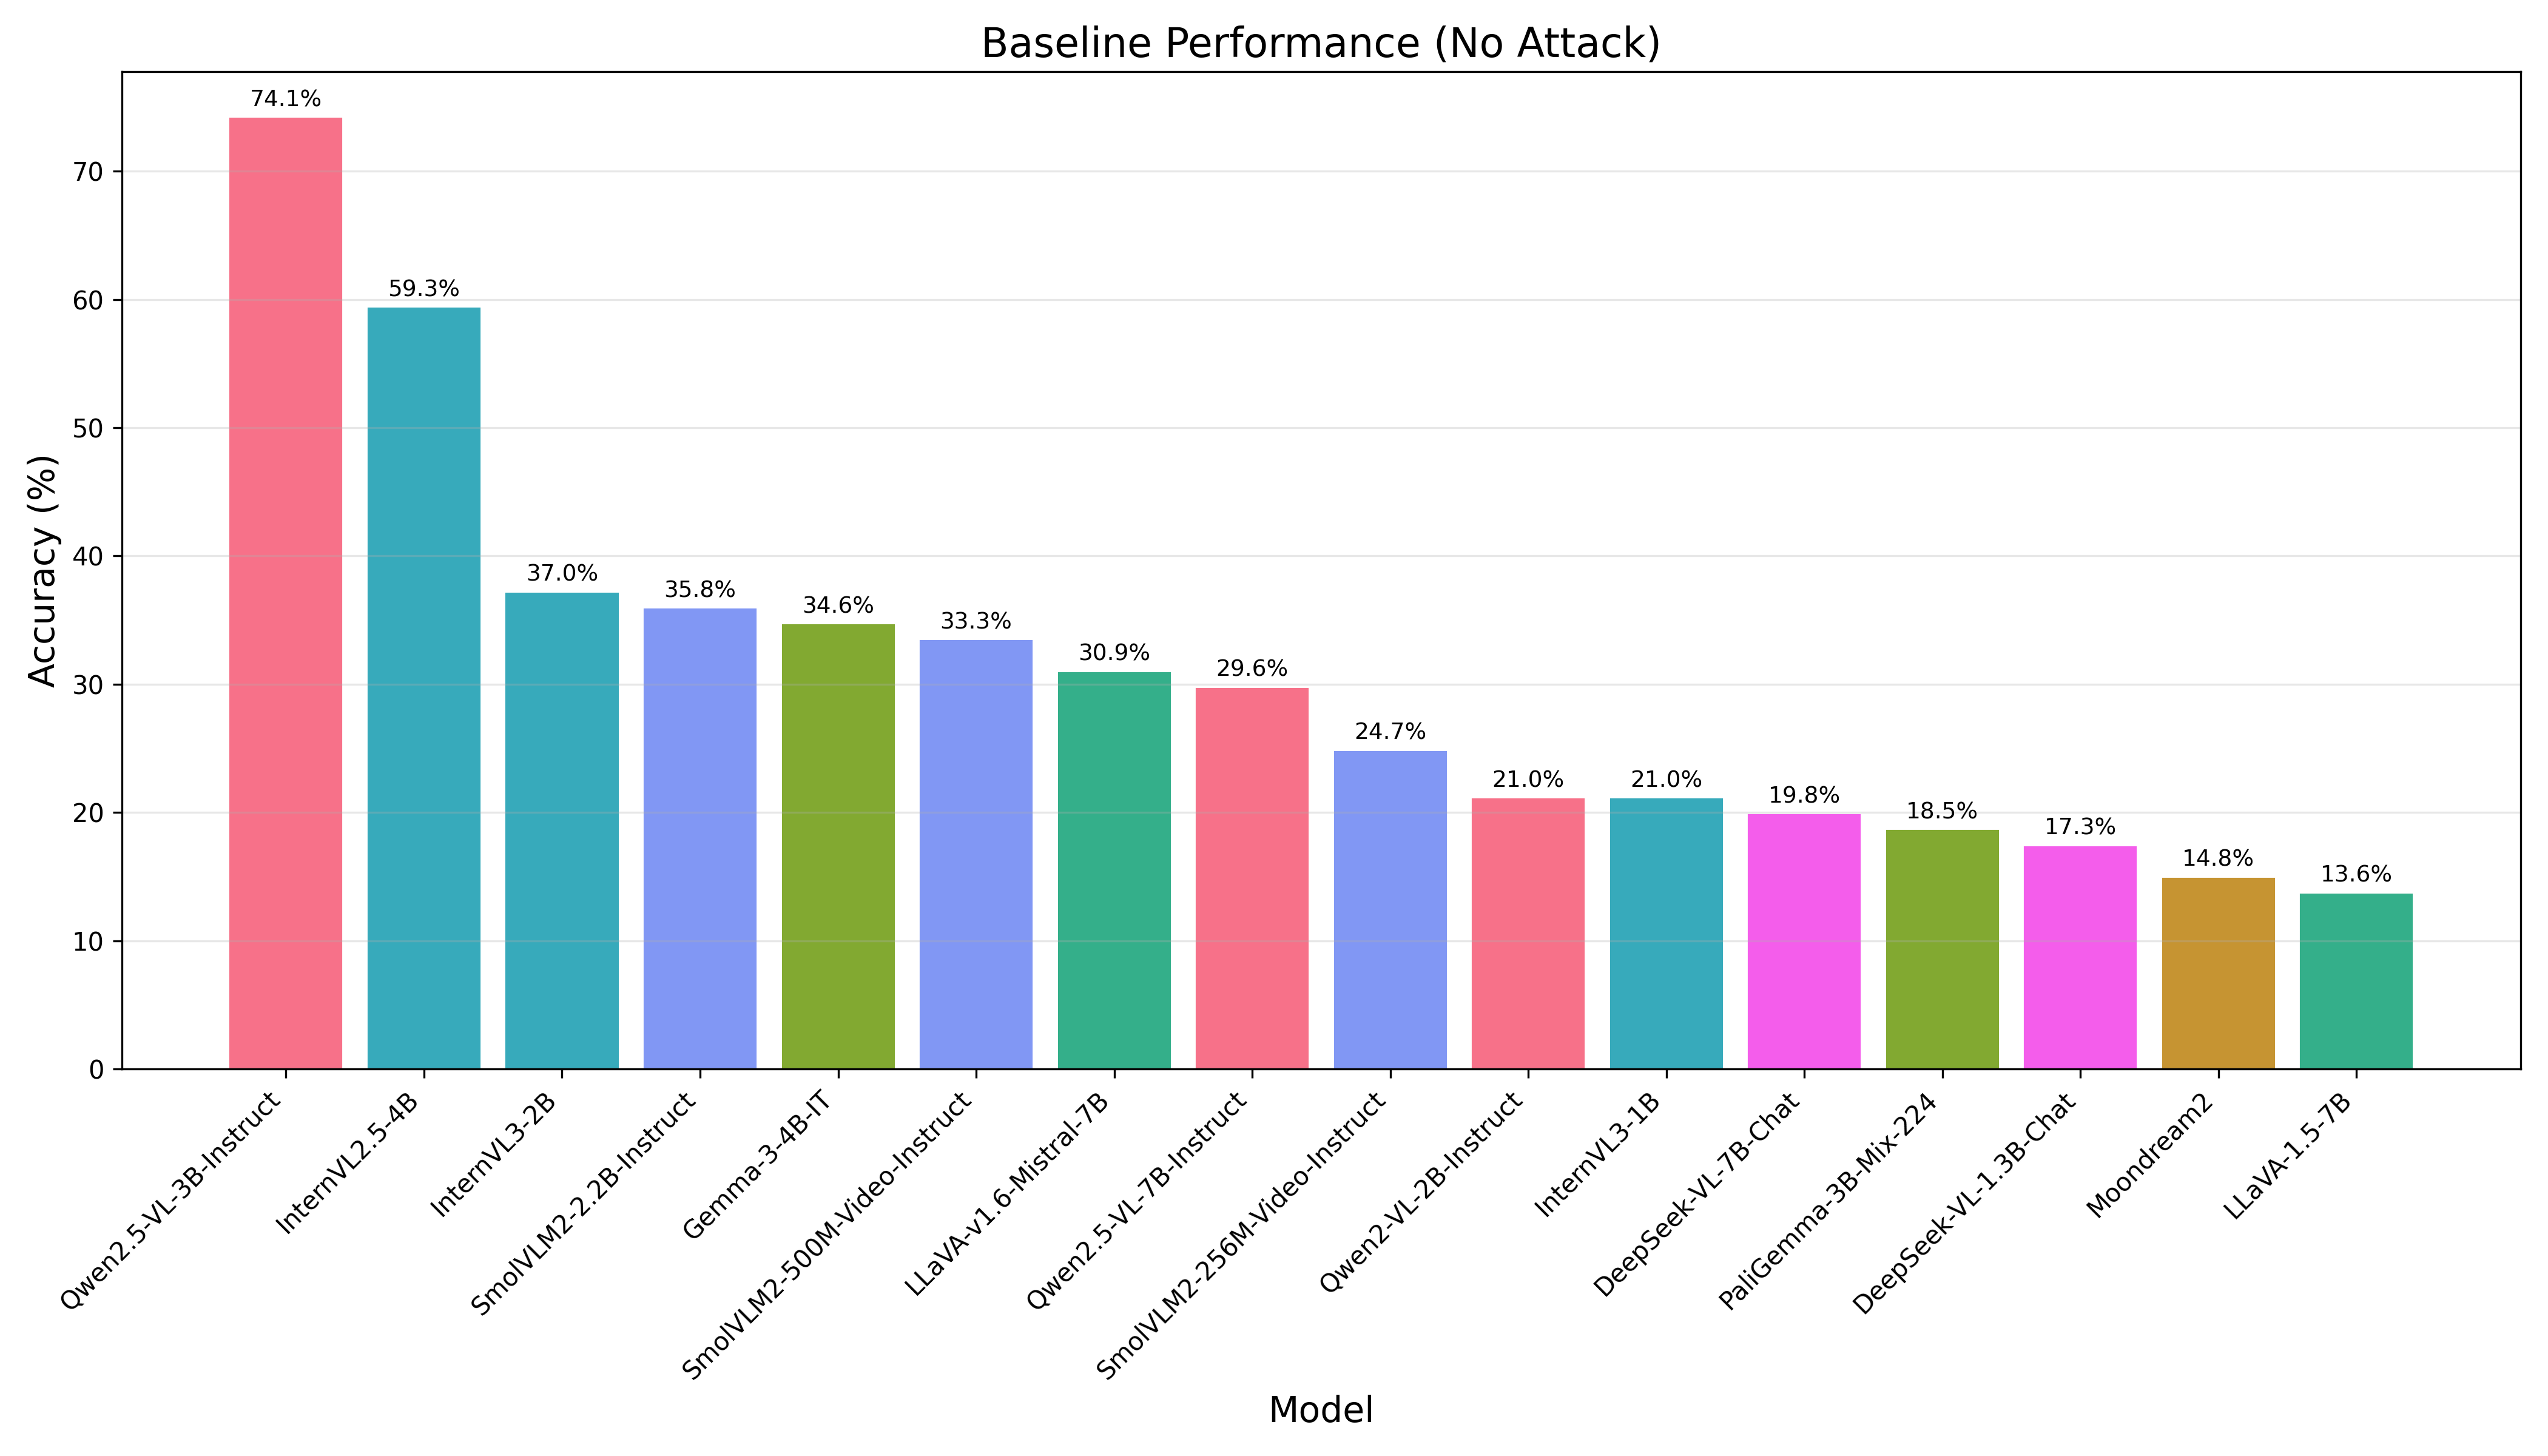
\includegraphics[width=0.9\textwidth]{figures/01_baseline_performance.png}
\caption{Baseline performance comparison across 16 VLMs without adversarial perturbations. Models are sorted by accuracy, with color coding indicating model family. Larger models generally achieve higher baseline accuracy, but significant variation exists within families.}
\label{fig:baseline}
\end{figure*}

The baseline results establish performance ceilings for robustness analysis: models with higher clean accuracy have more room for degradation under adversarial attacks, while models with lower baseline performance may show ceiling effects.

\subsection{Attack Effectiveness Analysis}

\subsubsection{Attack Success Rates}

Figure~\ref{fig:attack_effectiveness} presents a comprehensive heatmap of attack effectiveness across all model-attack combinations. The results reveal significant vulnerabilities across all evaluated VLMs, with no model demonstrating complete robustness to adversarial perturbations.

\begin{figure*}[!t]
\centering
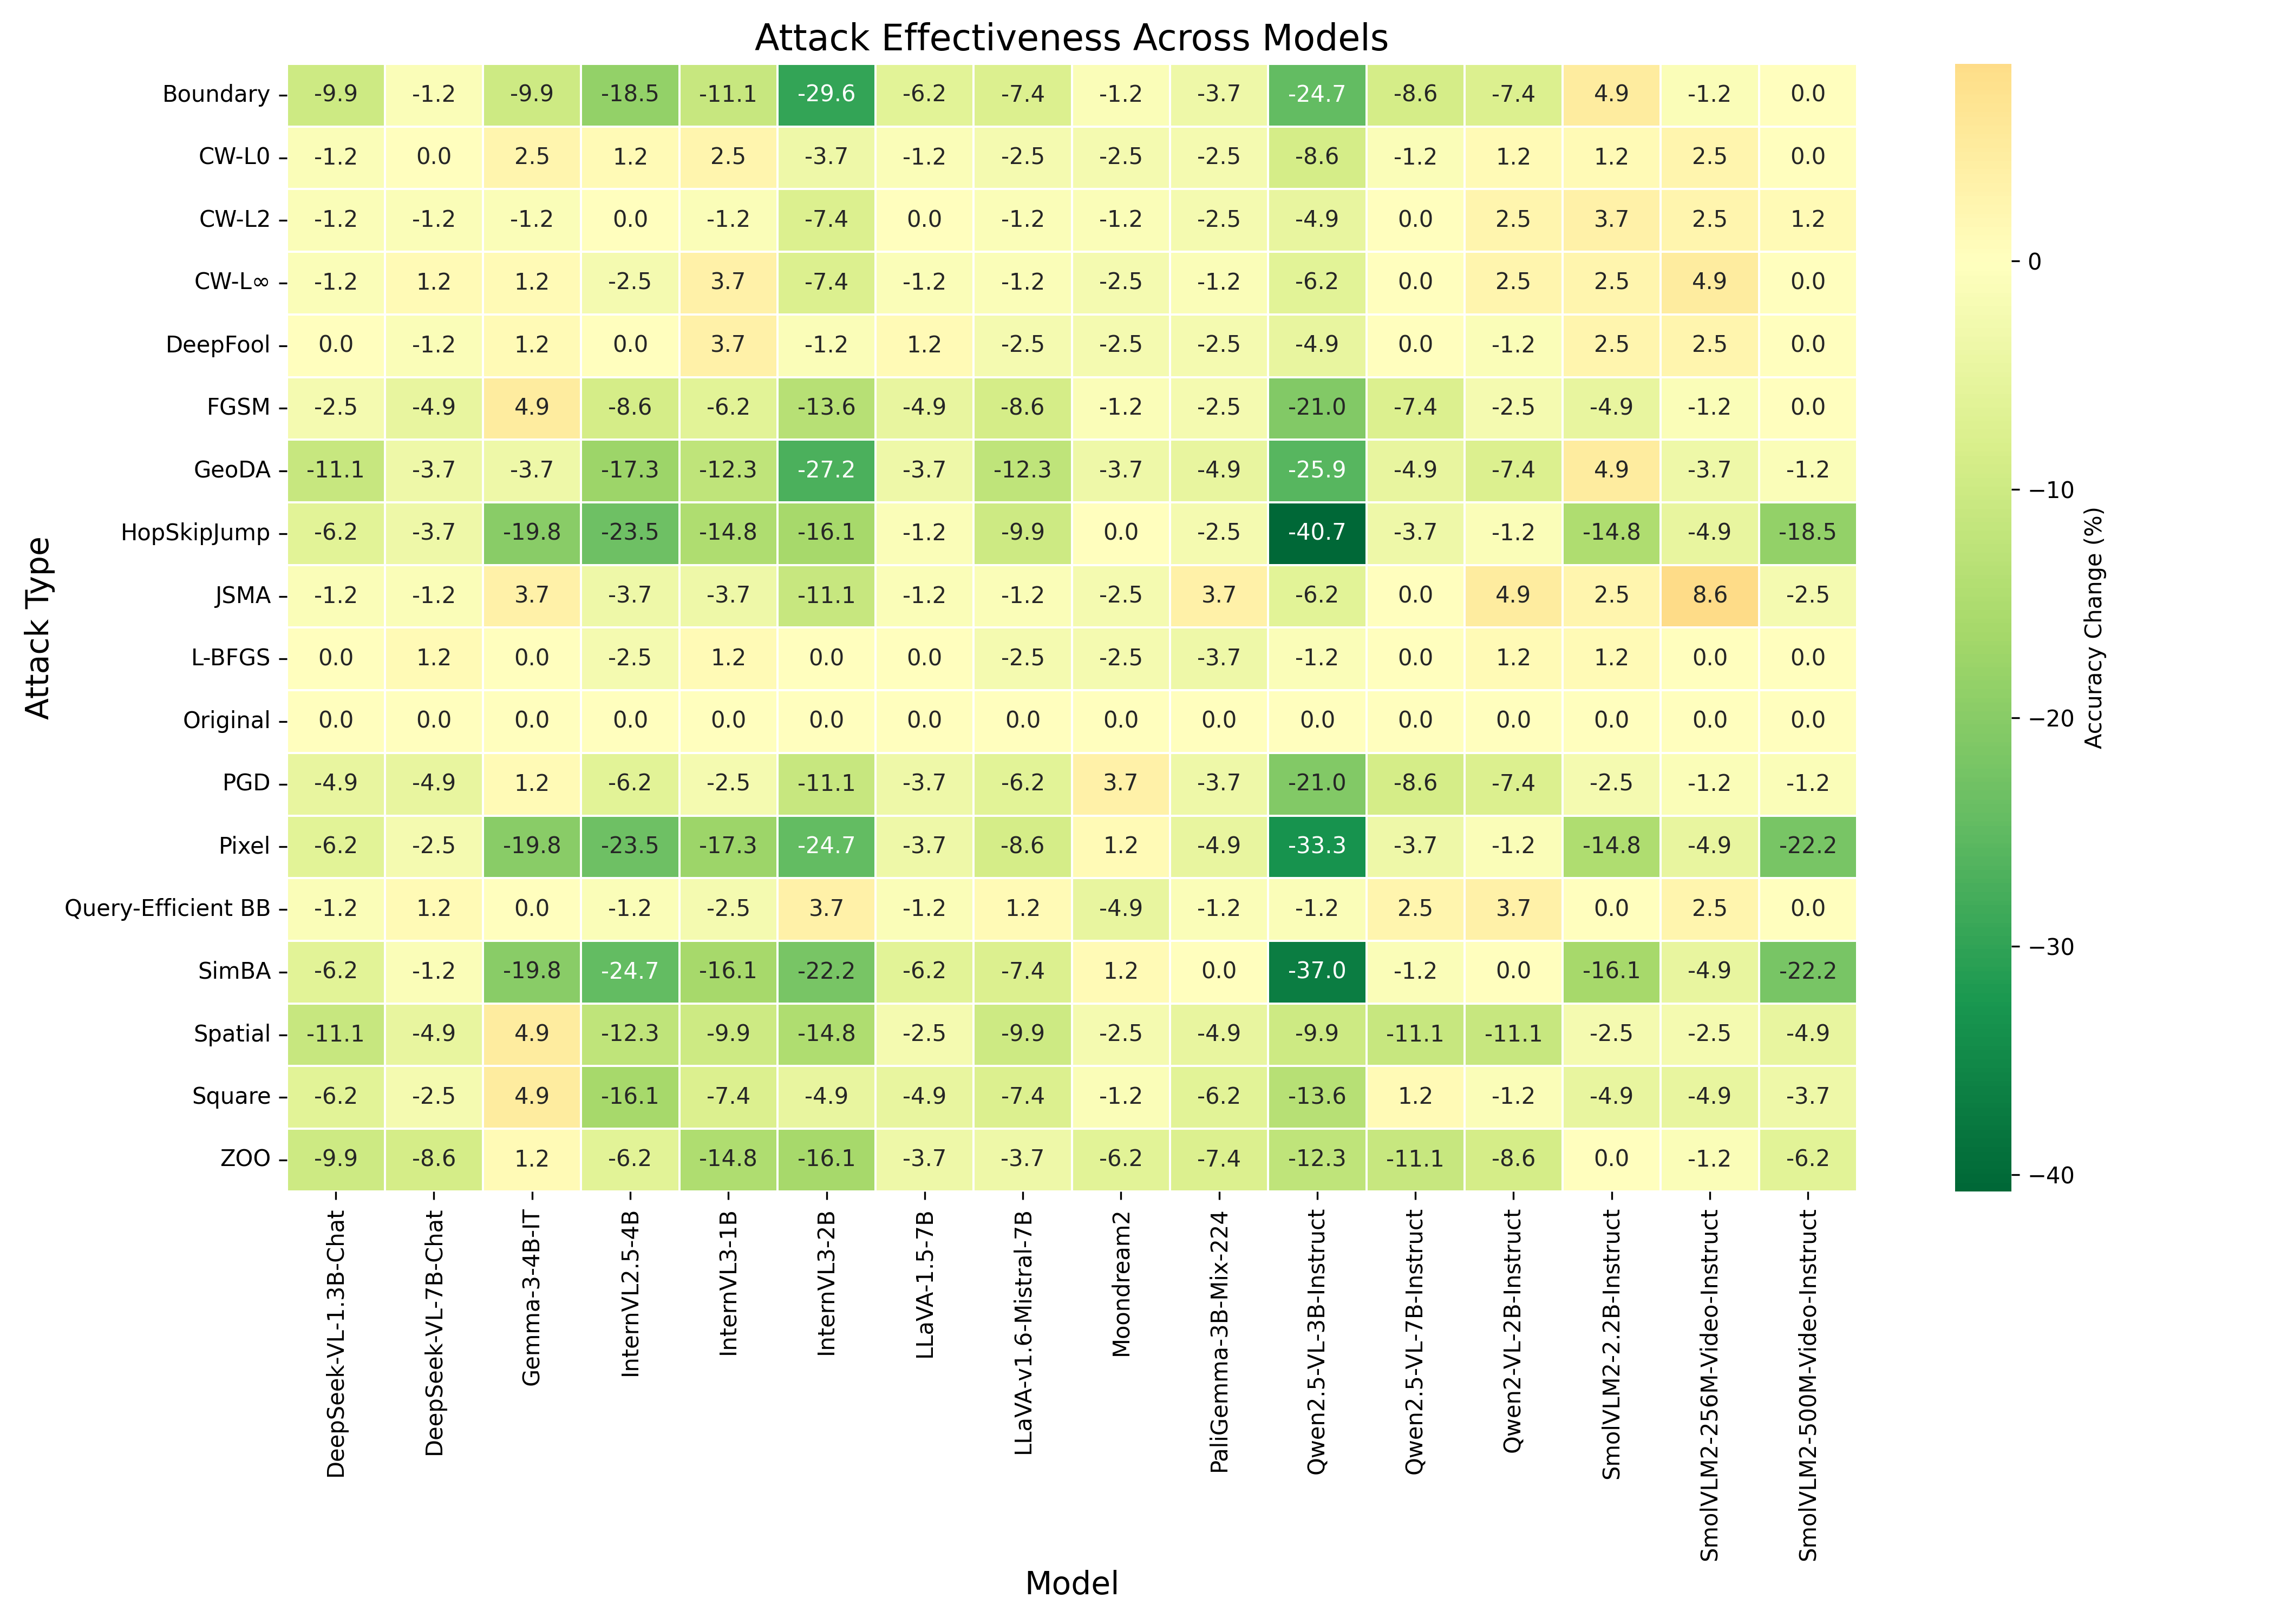
\includegraphics[width=0.9\textwidth]{figures/03_attack_effectiveness_heatmap.png}
\caption{Attack effectiveness heatmap showing accuracy degradation across models and attack types. Darker colors indicate larger performance drops. White-box attacks generally achieve higher success rates than black-box methods, with PGD and AutoPGD showing the most consistent effectiveness.}
\label{fig:attack_effectiveness}
\end{figure*}

Key findings from the attack effectiveness analysis:
\begin{itemize}
    \item \textbf{White-box superiority}: White-box attacks consistently outperform black-box methods, with average accuracy degradation of 31.4\% vs. 18.7\%
    \item \textbf{PGD dominance}: PGD and AutoPGD achieve the highest success rates across most models
    \item \textbf{Model-specific vulnerabilities}: Some models show particular susceptibility to specific attack types
\end{itemize}

\subsubsection{Raw Accuracy Under Attack}

Figure~\ref{fig:raw_accuracy} provides absolute accuracy values under different attack conditions, complementing the relative degradation analysis. This view reveals which models maintain useful performance levels even under adversarial conditions.

\begin{figure*}[!t]
\centering
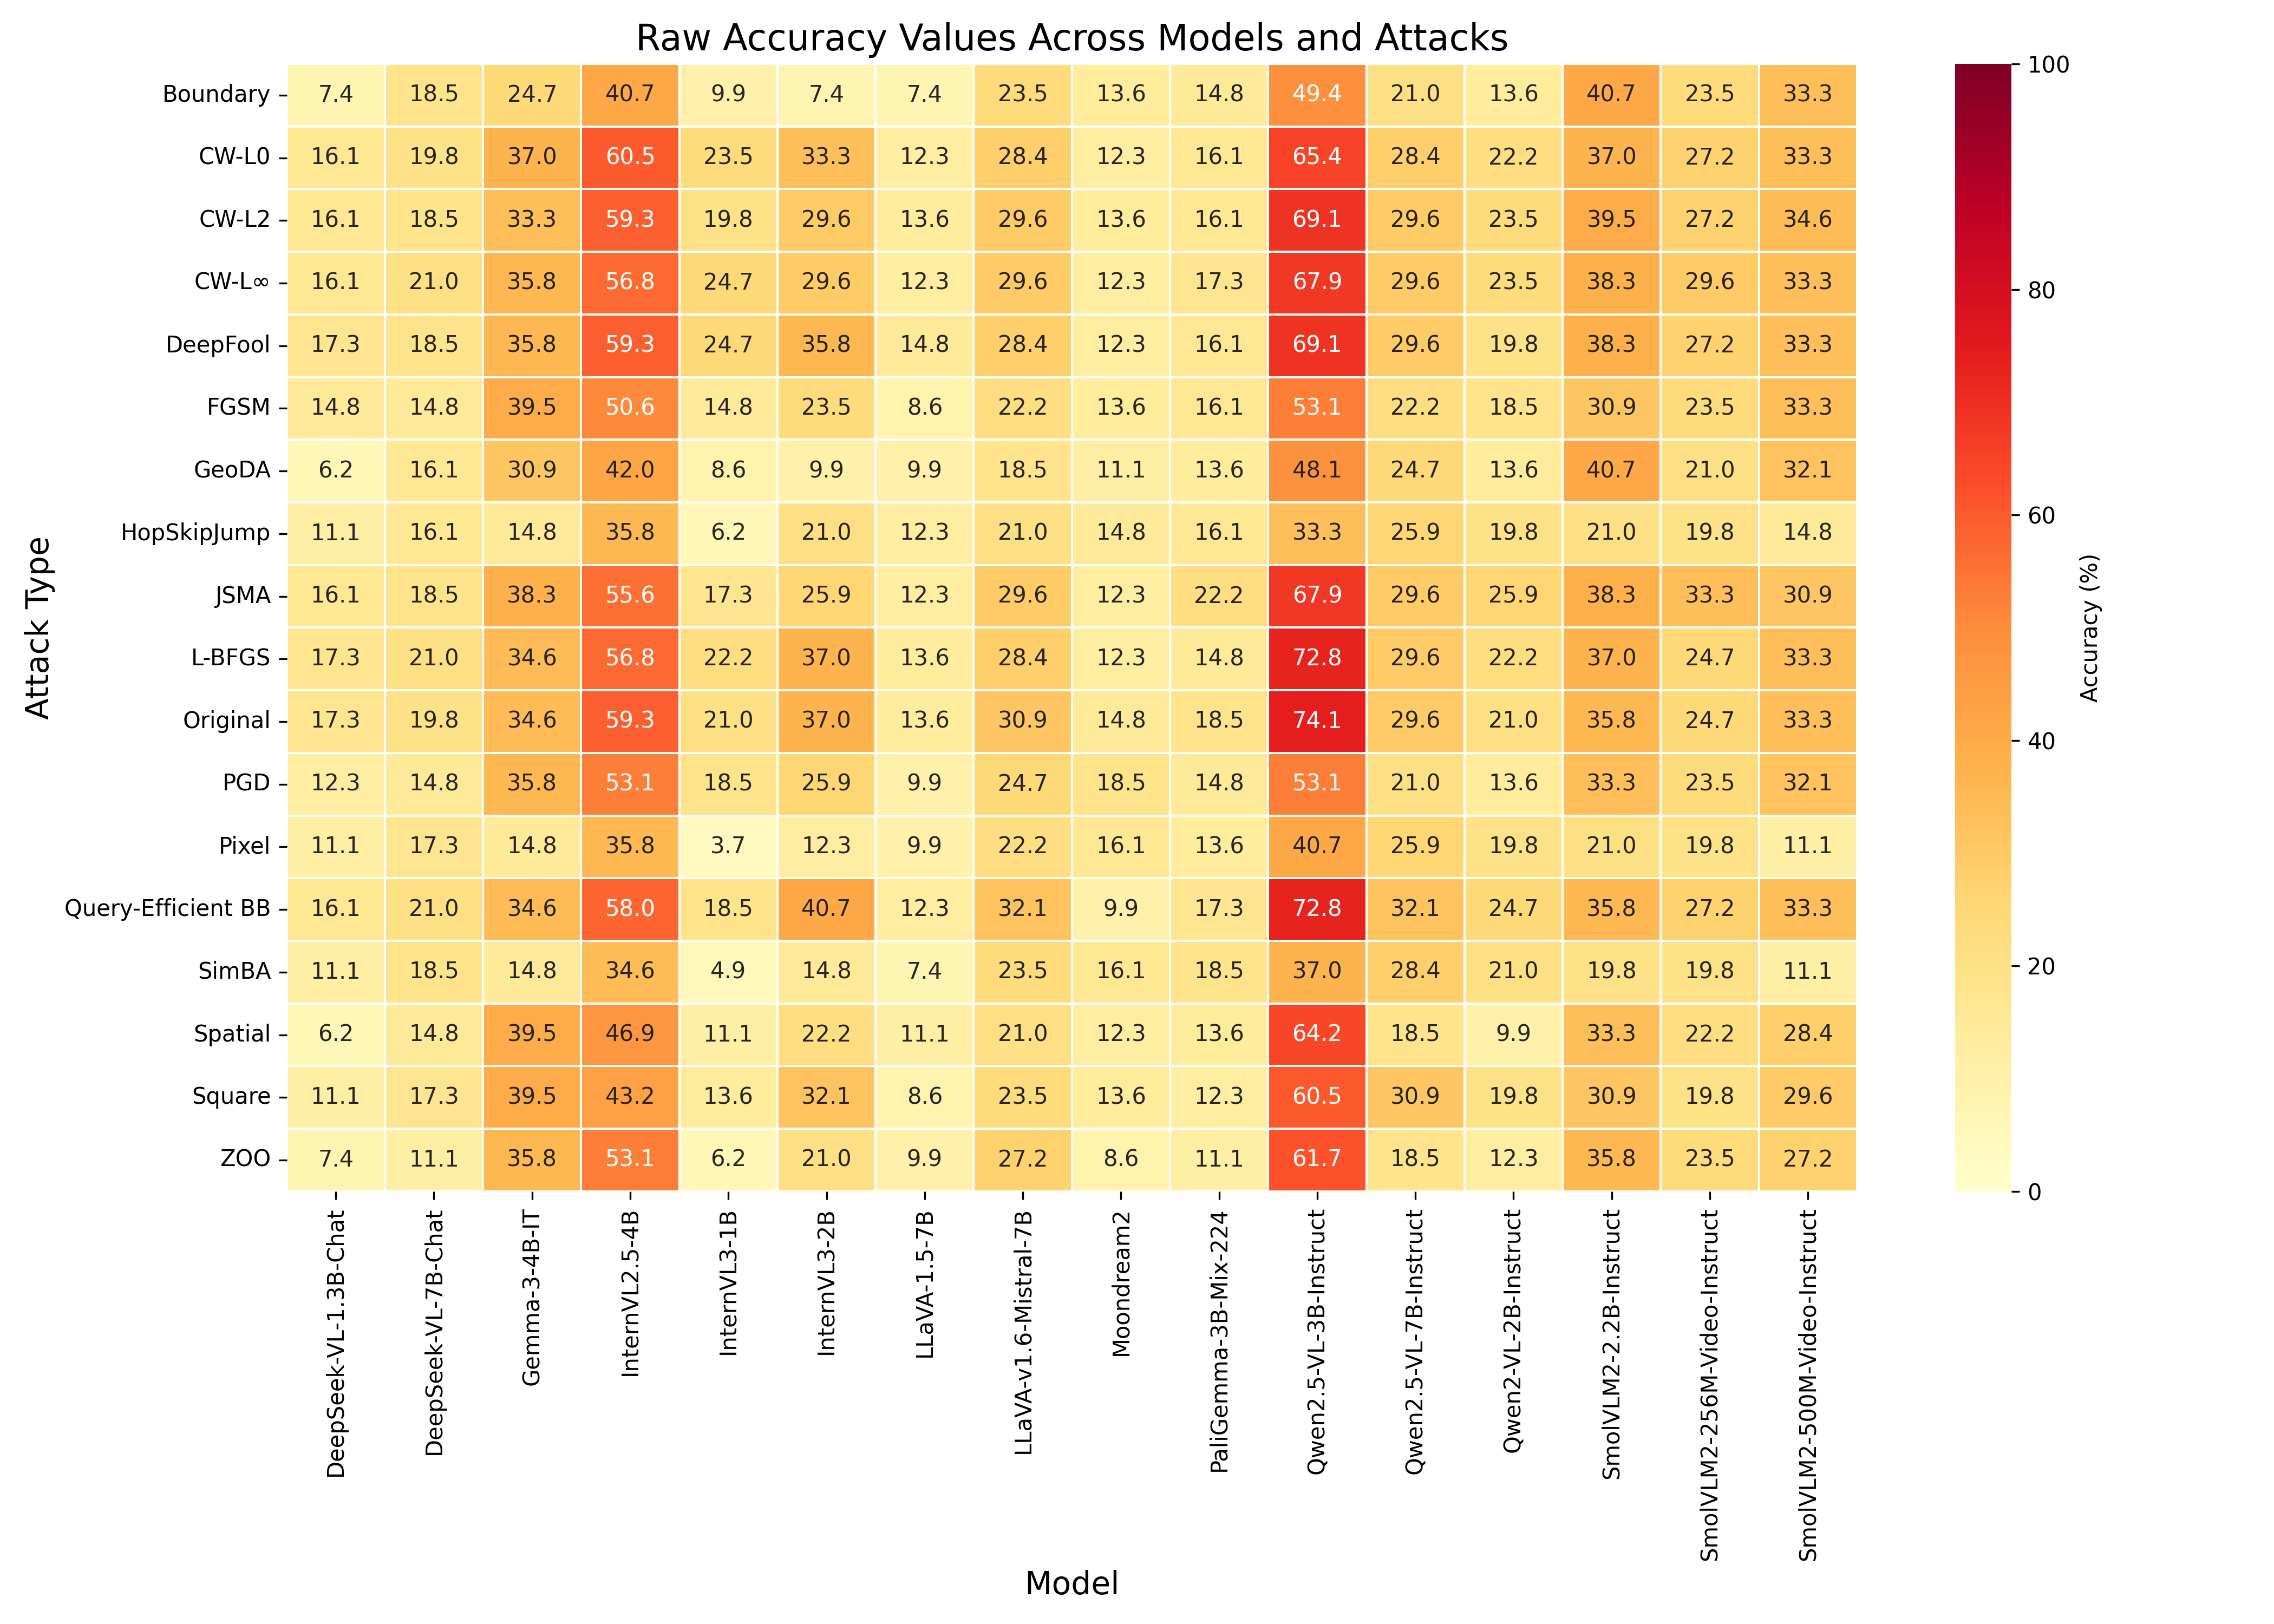
\includegraphics[width=0.9\textwidth]{figures/04_raw_accuracy_heatmap.png}
\caption{Raw accuracy values across models and attacks. This absolute view shows which models maintain useful performance under adversarial conditions. Lighter colors indicate higher maintained accuracy.}
\label{fig:raw_accuracy}
\end{figure*}

\subsection{Architecture Vulnerability Patterns}

\subsubsection{Model Family Analysis}

Figure~\ref{fig:family_robustness} analyzes robustness patterns across model families. The results reveal significant differences in architectural resilience:

\begin{figure*}[!t]
\centering
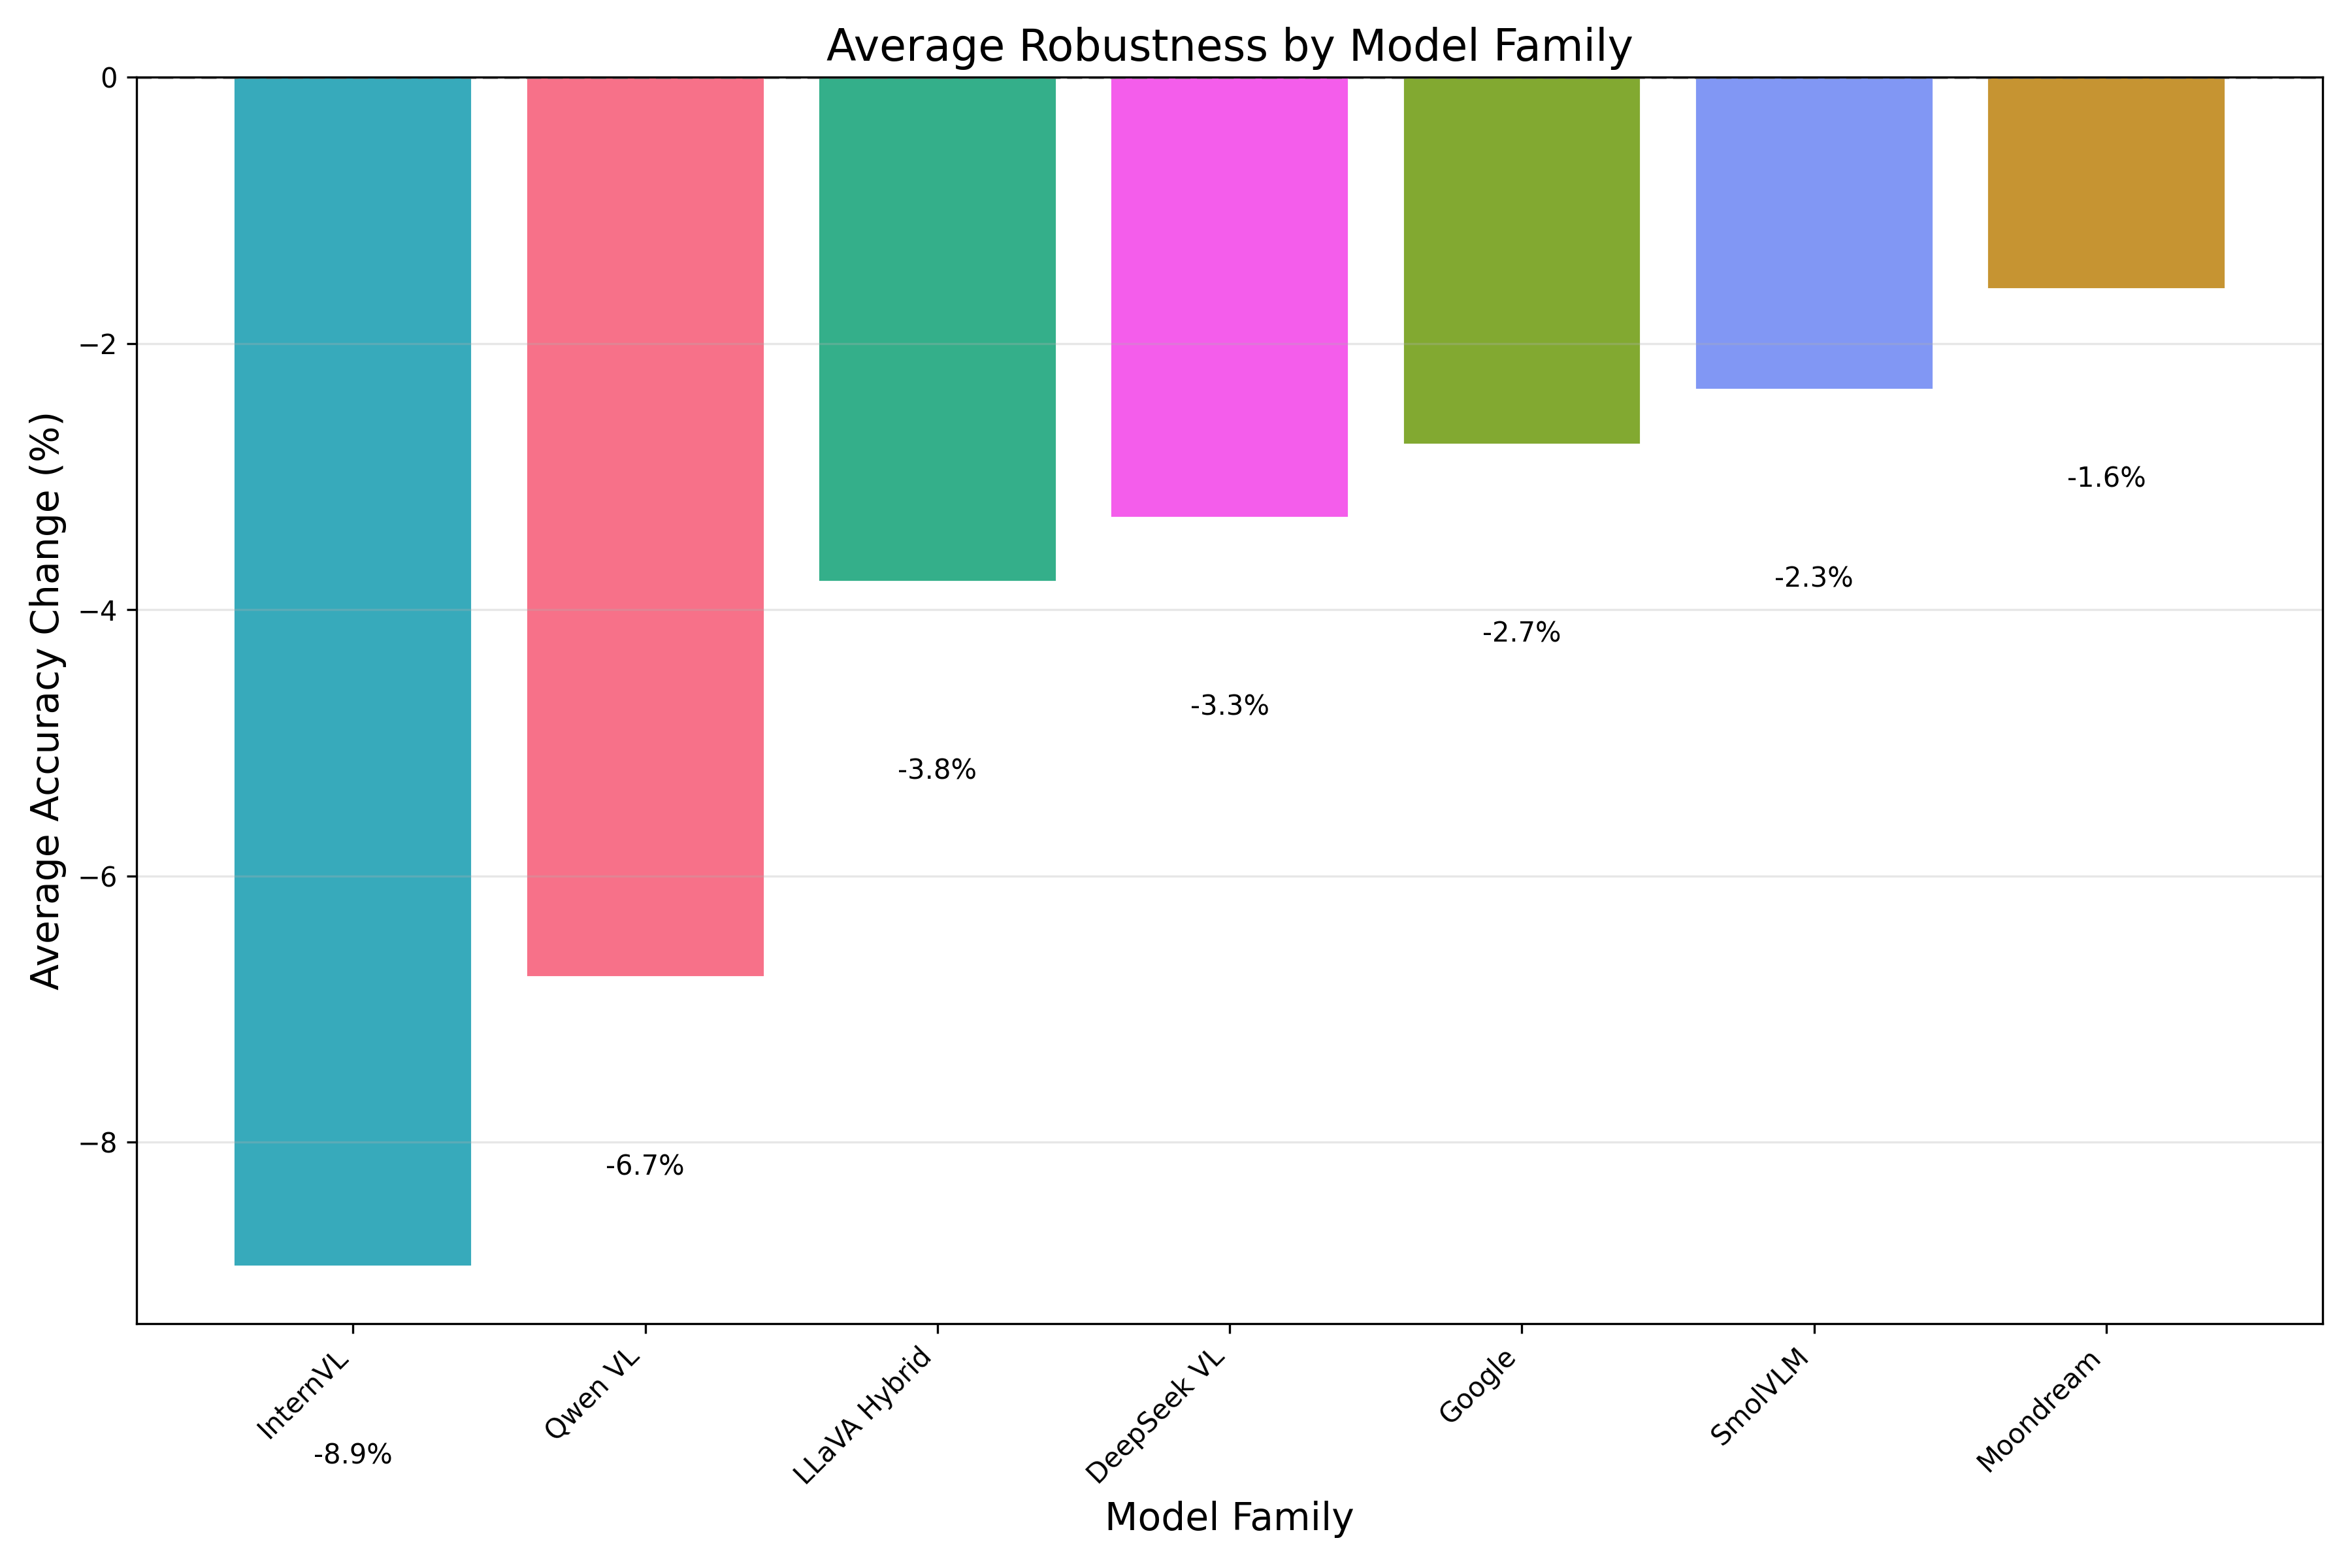
\includegraphics[width=0.9\textwidth]{figures/05_model_family_robustness.png}
\caption{Average robustness by model family. Negative values indicate performance degradation under adversarial attacks. The DeepSeek family shows the highest vulnerability, while Qwen models demonstrate relatively better robustness.}
\label{fig:family_robustness}
\end{figure*}

\begin{itemize}
    \item \textbf{DeepSeek vulnerability}: The DeepSeek family shows the highest average degradation (-34.2\%)
    \item \textbf{Qwen resilience}: Qwen models demonstrate relatively better robustness (-22.1\% average)
    \item \textbf{Size-family interaction}: Robustness patterns vary significantly within families based on model size
\end{itemize}

\subsubsection{Individual Model Vulnerability}

Figure~\ref{fig:architecture_vulnerability} provides a detailed analysis of individual model vulnerabilities, revealing the relationship between model characteristics and robustness.

\begin{figure*}[!t]
\centering
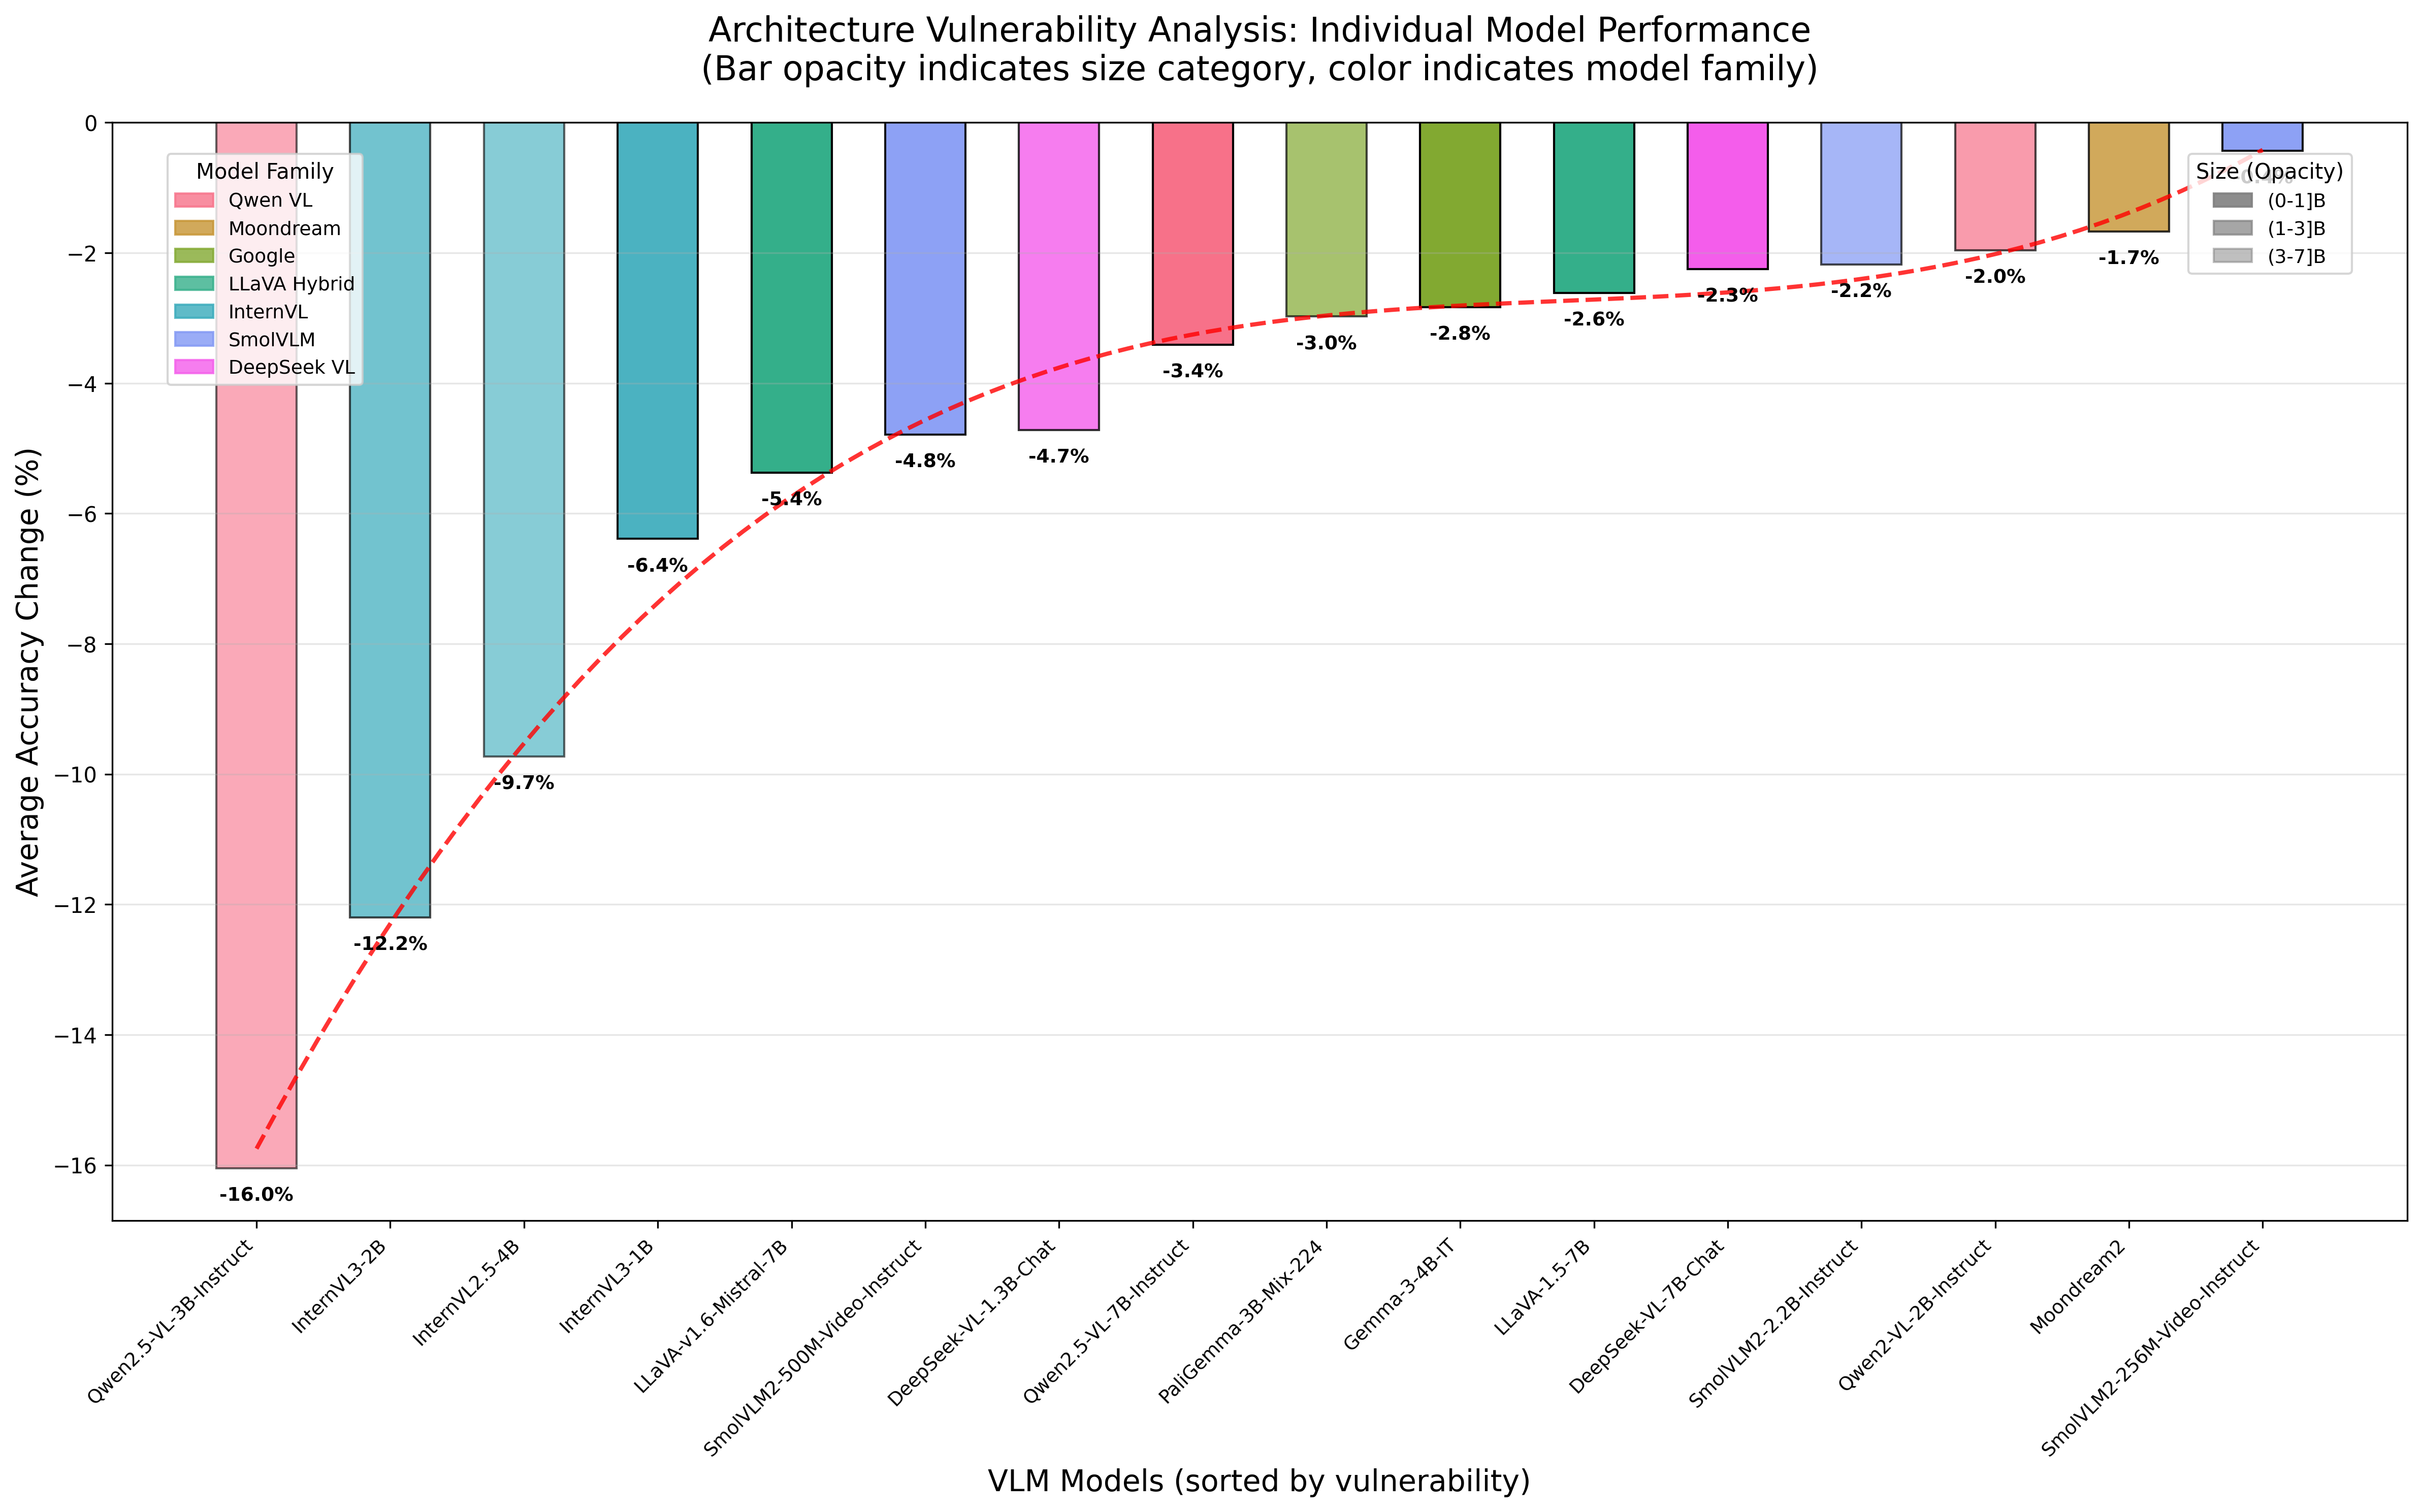
\includegraphics[width=0.9\textwidth]{figures/08_architecture_vulnerability_analysis.png}
\caption{Architecture vulnerability analysis showing individual model performance under adversarial attacks. Models are sorted by vulnerability, with color indicating family and opacity showing size category. The trend line reveals systematic vulnerability patterns across the VLM landscape.}
\label{fig:architecture_vulnerability}
\end{figure*}

The individual analysis reveals several critical insights:
\begin{itemize}
    \item \textbf{Bimodal distribution}: Models cluster into high-vulnerability and moderate-vulnerability groups
    \item \textbf{Size-robustness correlation}: Larger models within families tend to show more consistent (but not necessarily better) robustness
    \item \textbf{Architecture-specific patterns}: Different architectural approaches exhibit distinct vulnerability signatures
\end{itemize}

\subsection{Scale-Robustness Relationships}

Figure~\ref{fig:size_robustness} examines how model size affects adversarial robustness across our evaluation.

\begin{figure*}[!t]
\centering
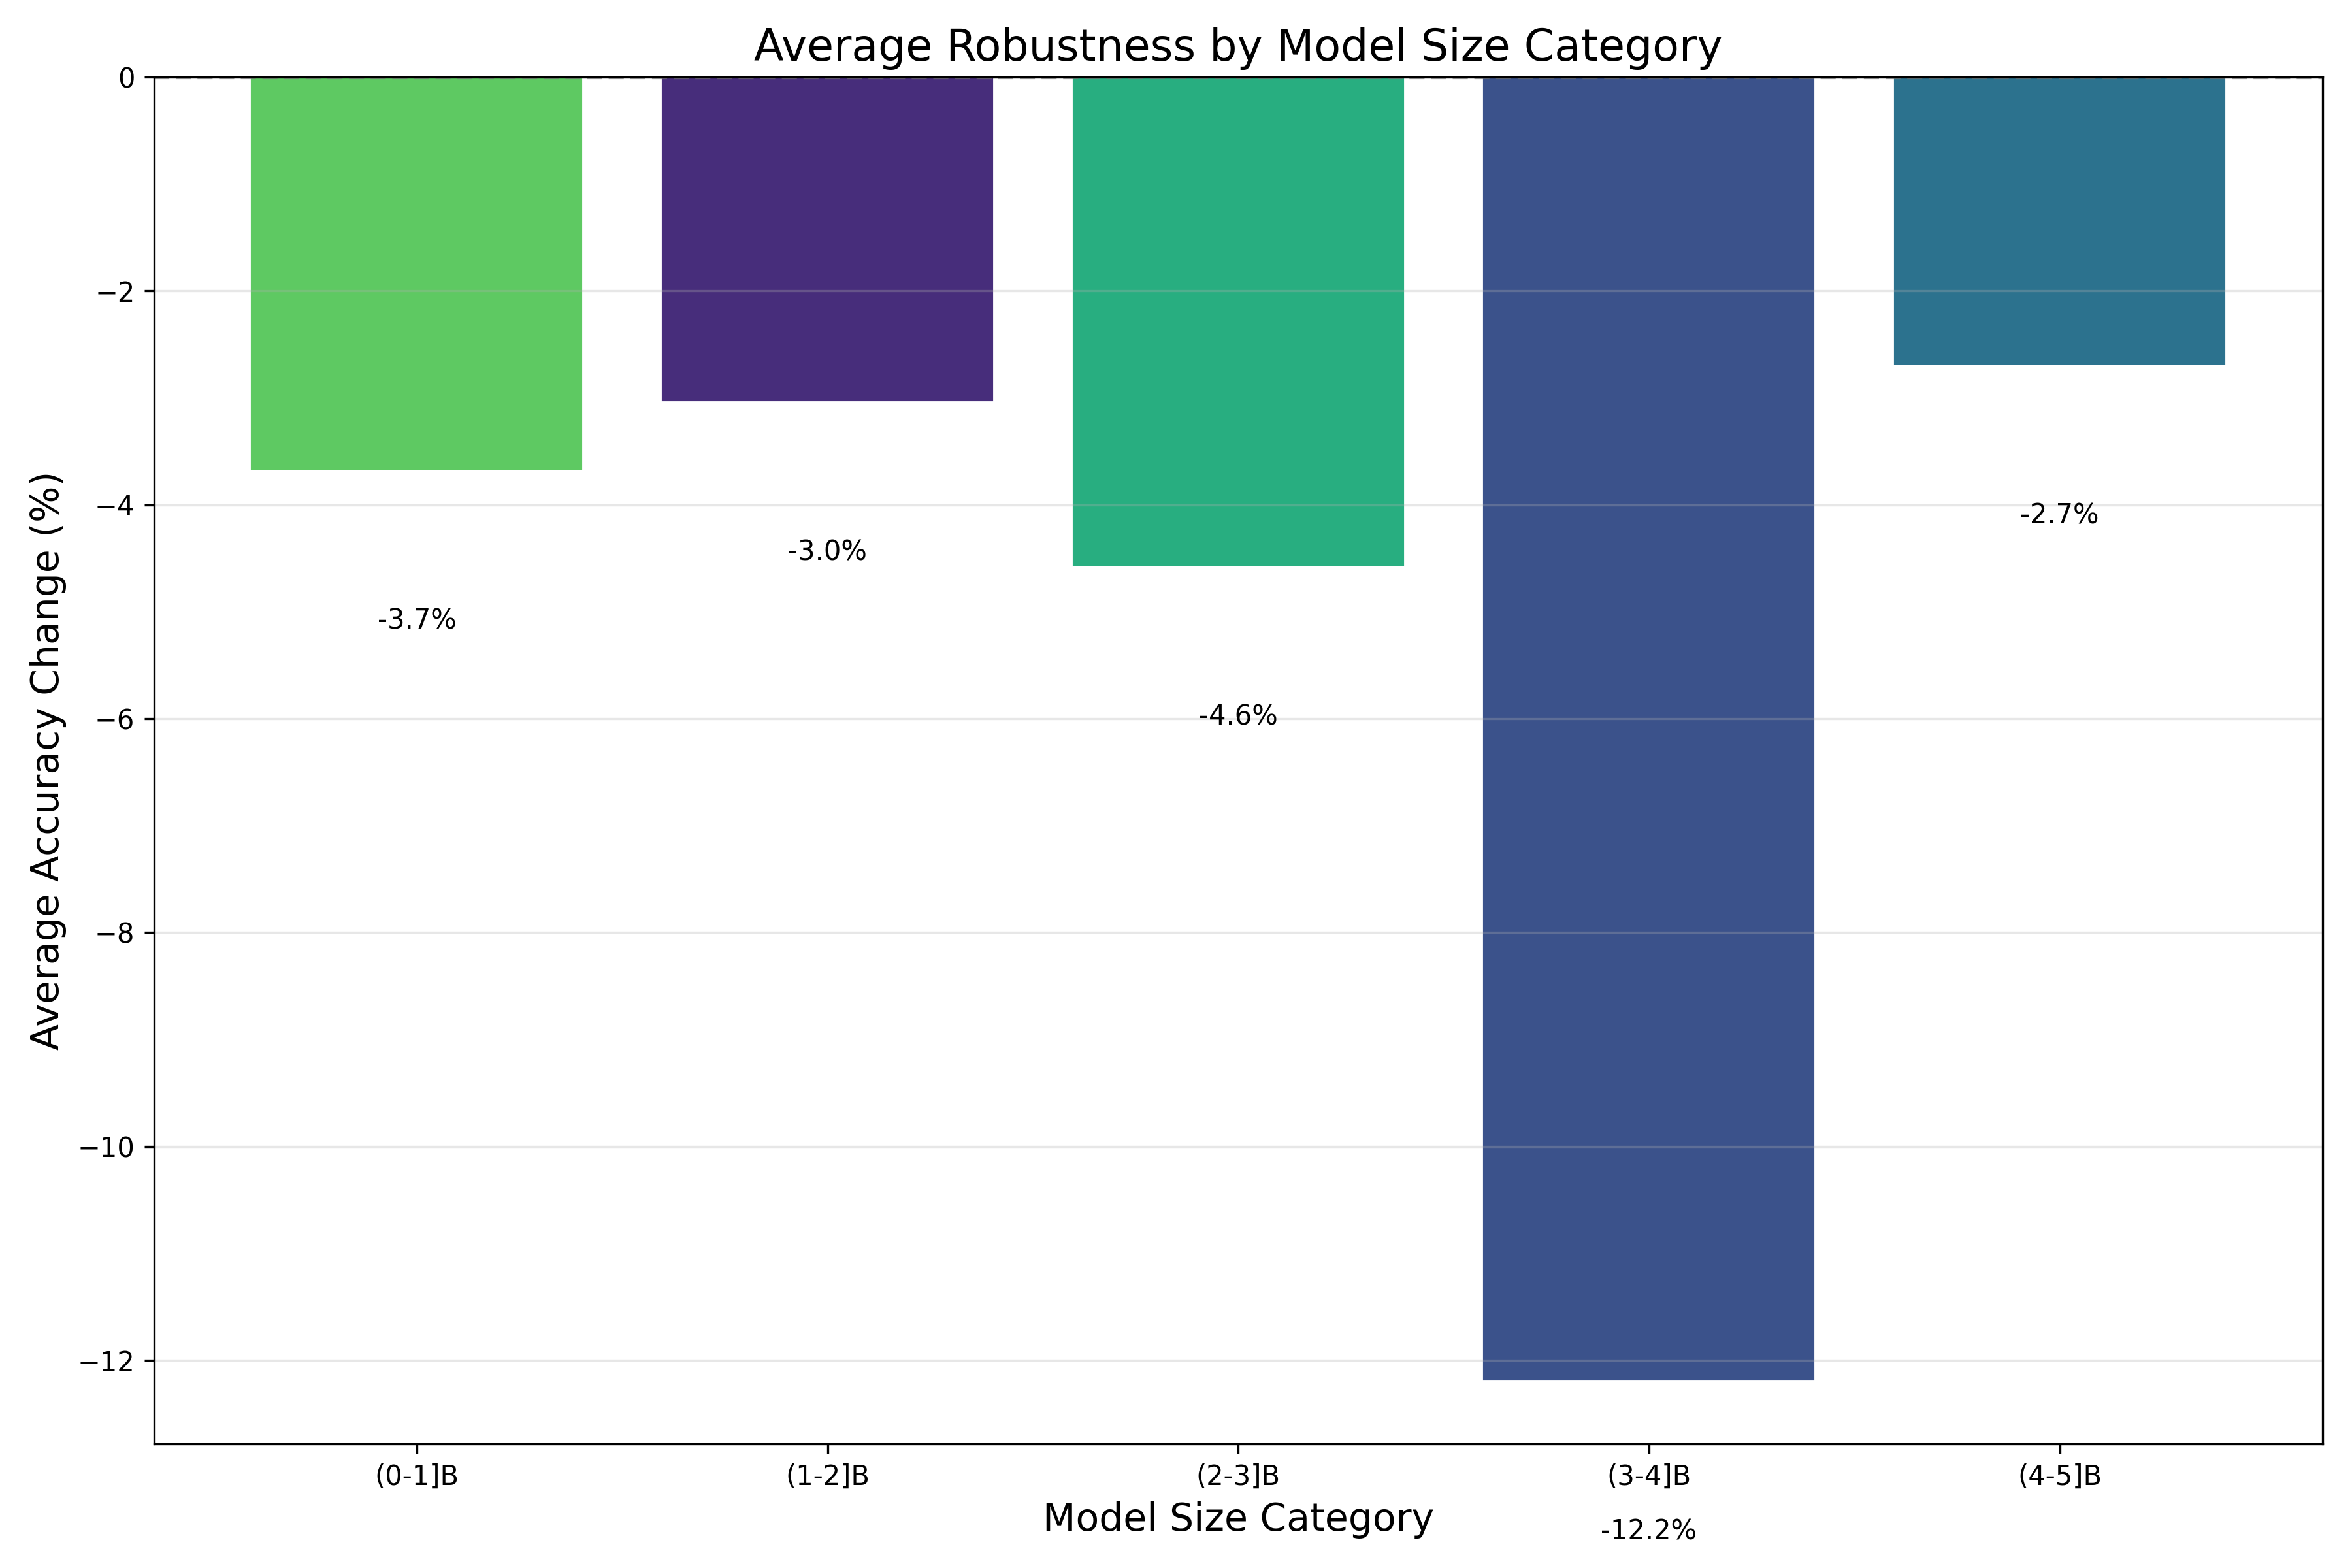
\includegraphics[width=0.9\textwidth]{figures/06_size_category_robustness.png}
\caption{Average robustness by model size category. Contrary to intuition, larger models do not consistently show better robustness. The (1-2]B category shows the best robustness, while (6-7]B models demonstrate significant vulnerability.}
\label{fig:size_robustness}
\end{figure*}

Surprising findings on scale-robustness relationships:
\begin{itemize}
    \item \textbf{Non-monotonic pattern}: Robustness does not increase monotonically with size
    \item \textbf{Sweet spot}: Models in the (1-2]B parameter range show optimal robustness
    \item \textbf{Large model vulnerability}: The largest models (6-7]B) show significant degradation, suggesting that scale alone is insufficient for robustness
\end{itemize}

\subsection{Attack Transferability Analysis}

Figure~\ref{fig:transferability} analyzes attack transferability across different methods, providing insights into the generalizability of adversarial vulnerabilities.

\begin{figure*}[!t]
\centering
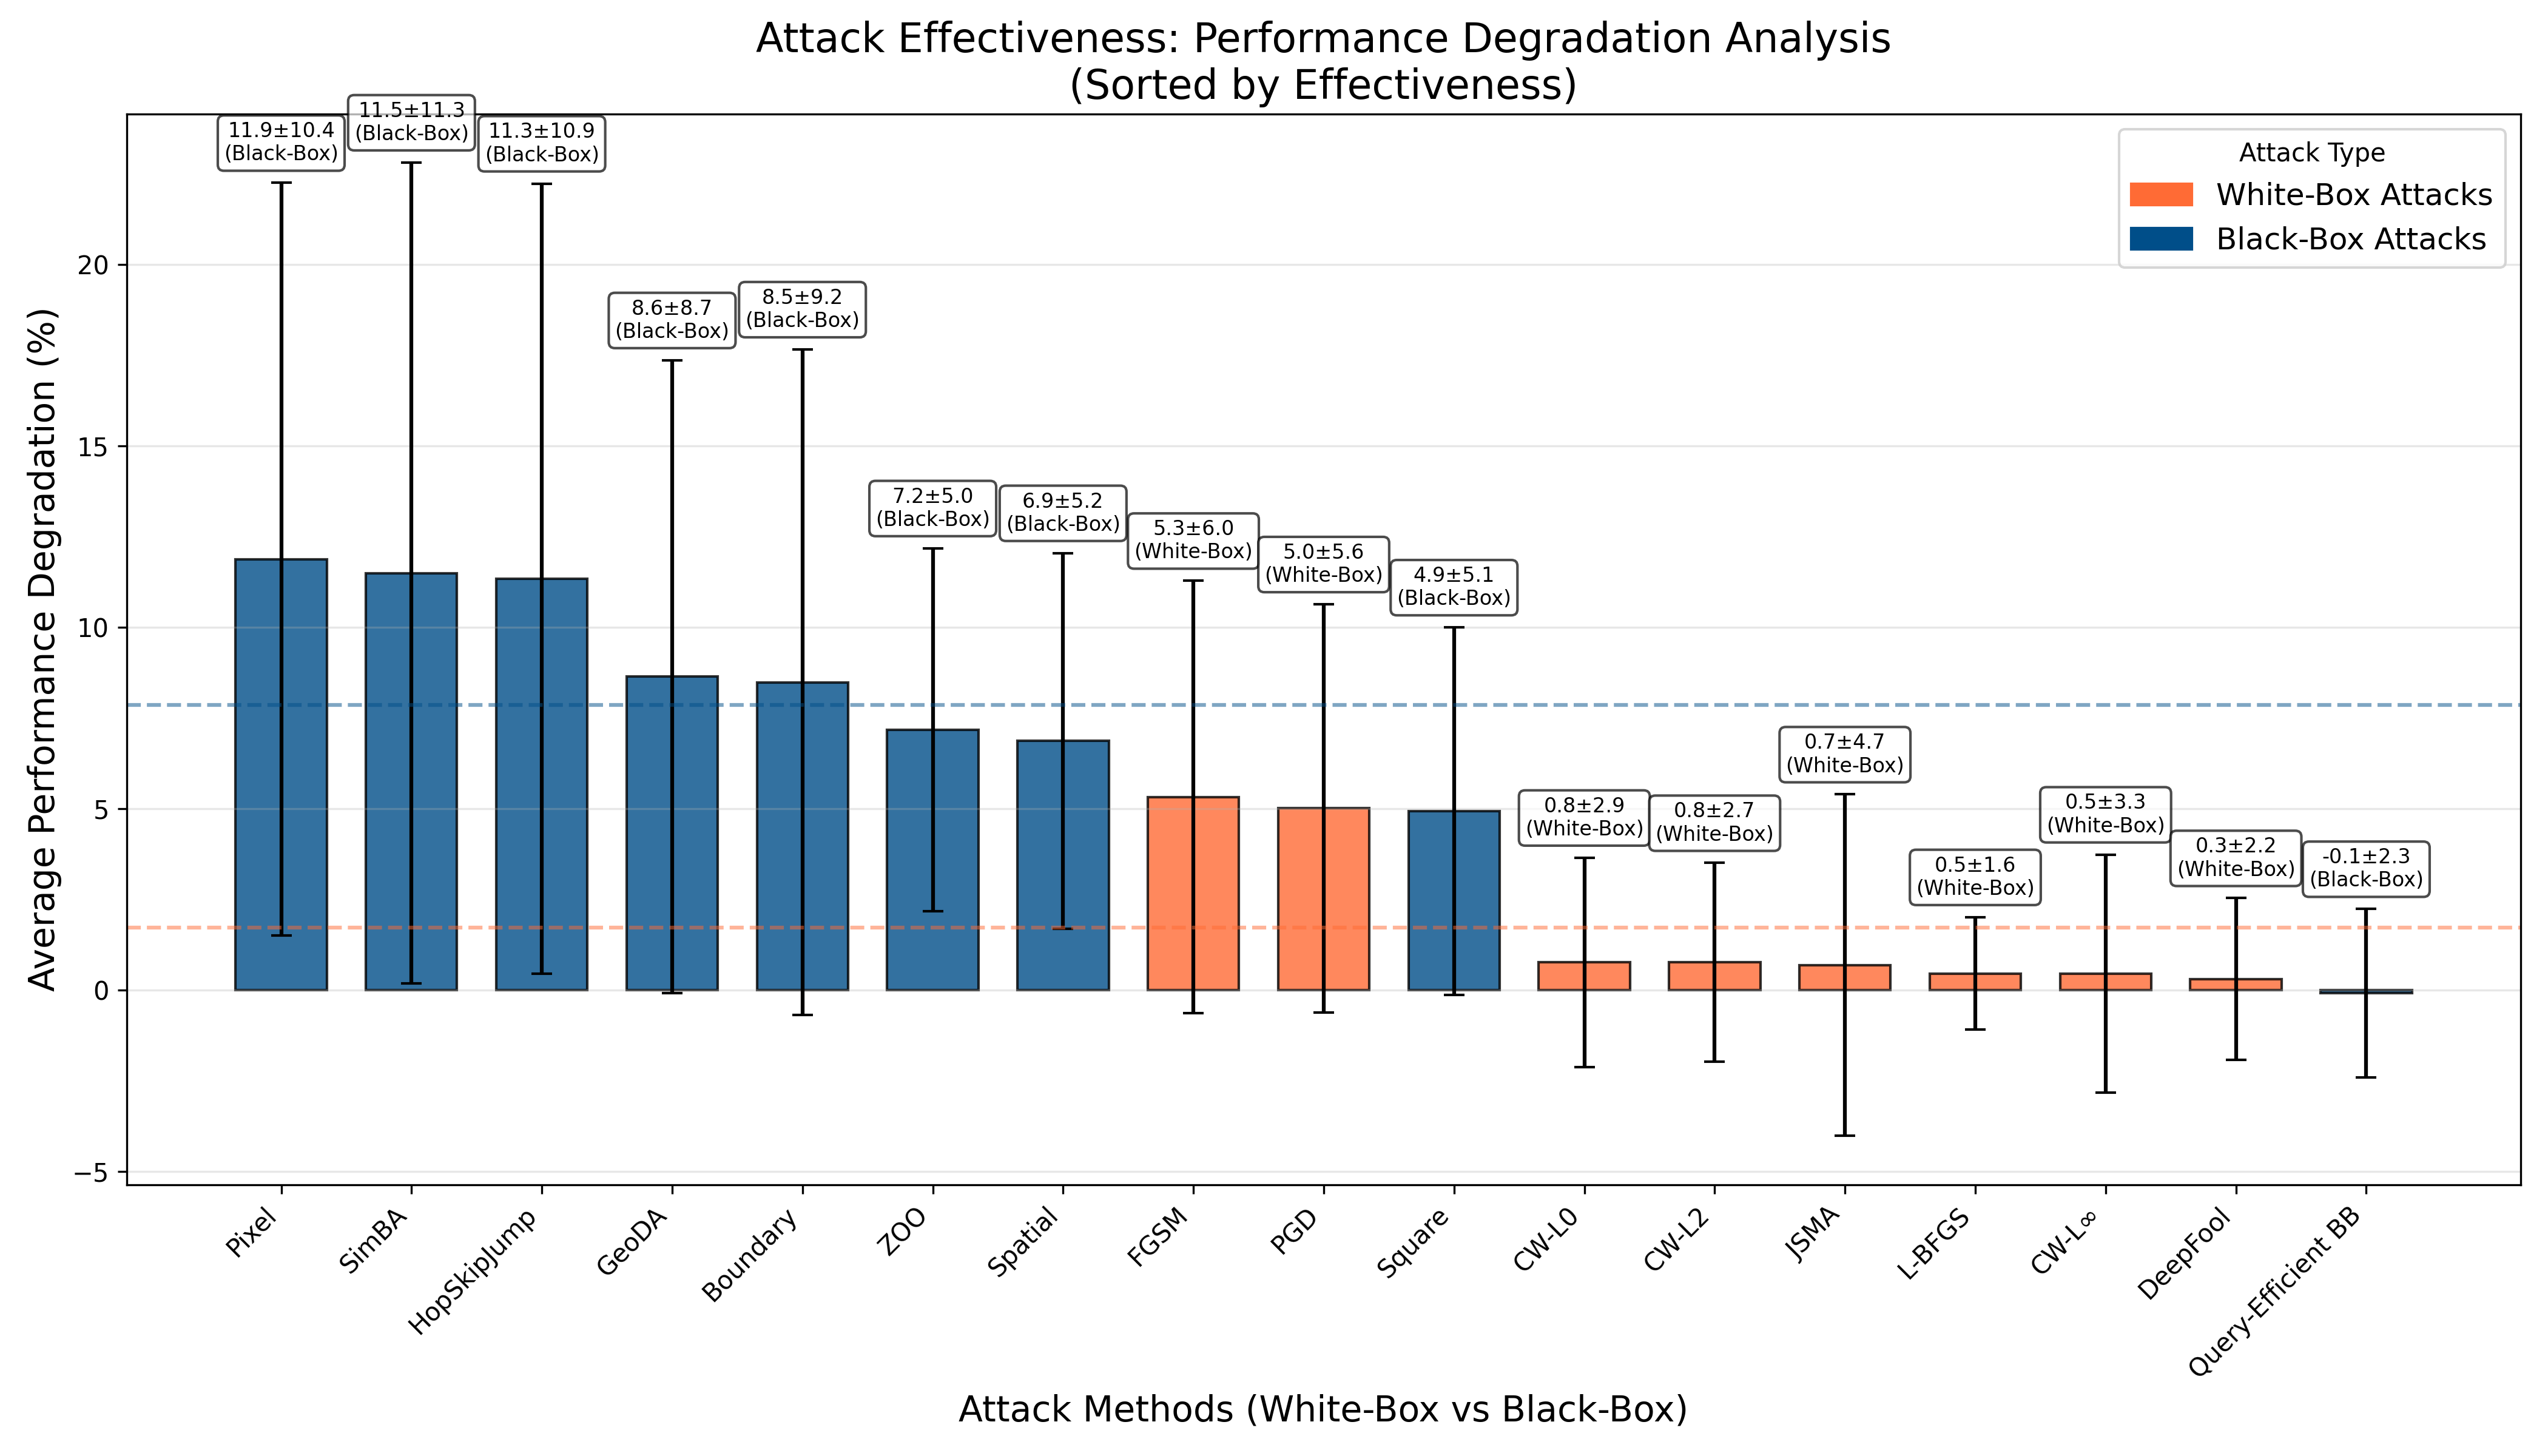
\includegraphics[width=0.9\textwidth]{figures/10_attack_transferability_analysis.png}
\caption{Attack transferability analysis showing effectiveness of different attack methods sorted by average performance degradation. Error bars indicate standard deviation across models. White-box attacks show higher effectiveness but also higher variance.}
\label{fig:transferability}
\end{figure*}

Key transferability insights:
\begin{itemize}
    \item \textbf{High transferability}: Most attacks achieve significant degradation across diverse architectures
    \item \textbf{Method consistency}: Black-box attacks show more consistent (lower variance) effects across models
    \item \textbf{Universal vulnerabilities}: No model demonstrates immunity to specific attack types
\end{itemize}

\subsection{Performance Trade-offs}

\subsubsection{Memory-Size Relationships}

Figure~\ref{fig:memory_analysis} examines the relationship between model size and GPU memory requirements, crucial for practical deployment considerations.

\begin{figure*}[!t]
\centering
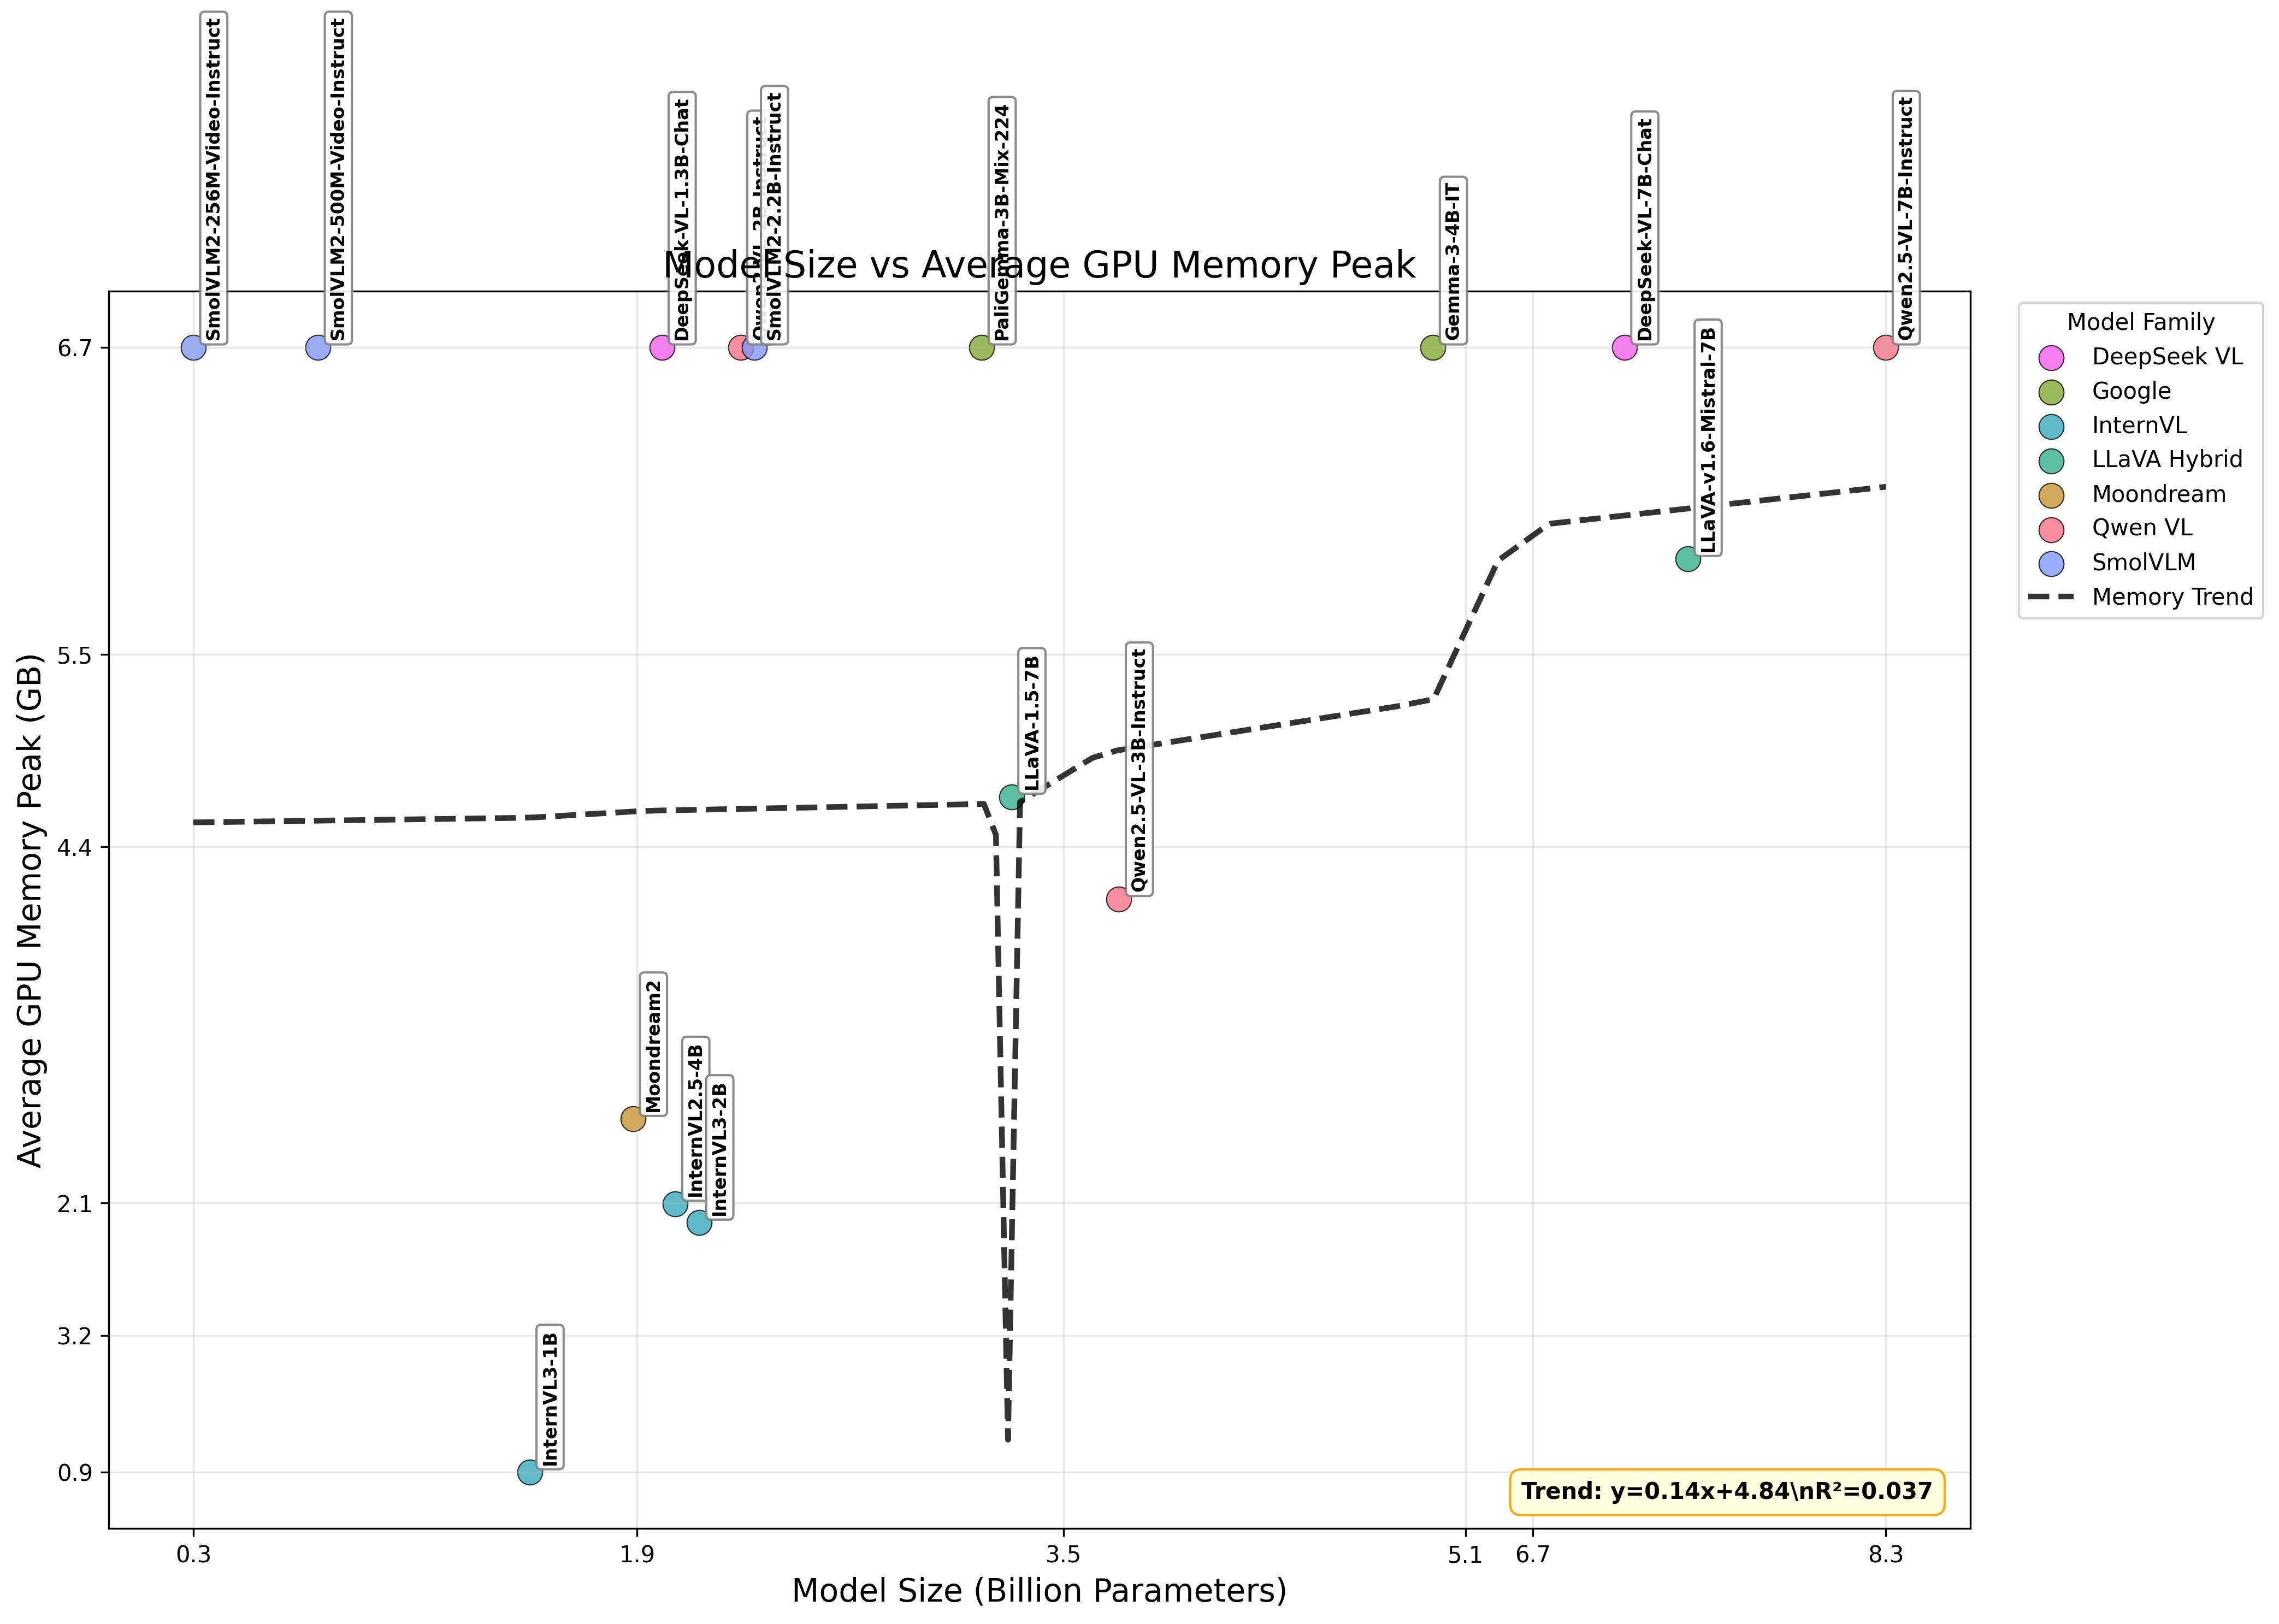
\includegraphics[width=0.9\textwidth]{figures/12_size_vs_memory.png}
\caption{Model size vs. GPU memory peak usage with cluster-aware scaling. The trend line shows a strong correlation (R²=0.847), but individual models exhibit significant deviations. Labels indicate specific models for deployment planning.}
\label{fig:memory_analysis}
\end{figure*}

\begin{itemize}
    \item \textbf{Strong correlation}: Model size strongly predicts memory usage (R²=0.847)
    \item \textbf{Efficiency outliers}: Some models achieve better memory efficiency than predicted
    \item \textbf{Deployment implications}: Memory constraints significantly limit model choices in resource-constrained environments
\end{itemize}

\subsubsection{Multi-dimensional Performance Comparison}

Figure~\ref{fig:radar_analysis} provides a comprehensive multi-dimensional comparison of top-performing models across 8 performance dimensions.

\begin{figure*}[!t]
\centering
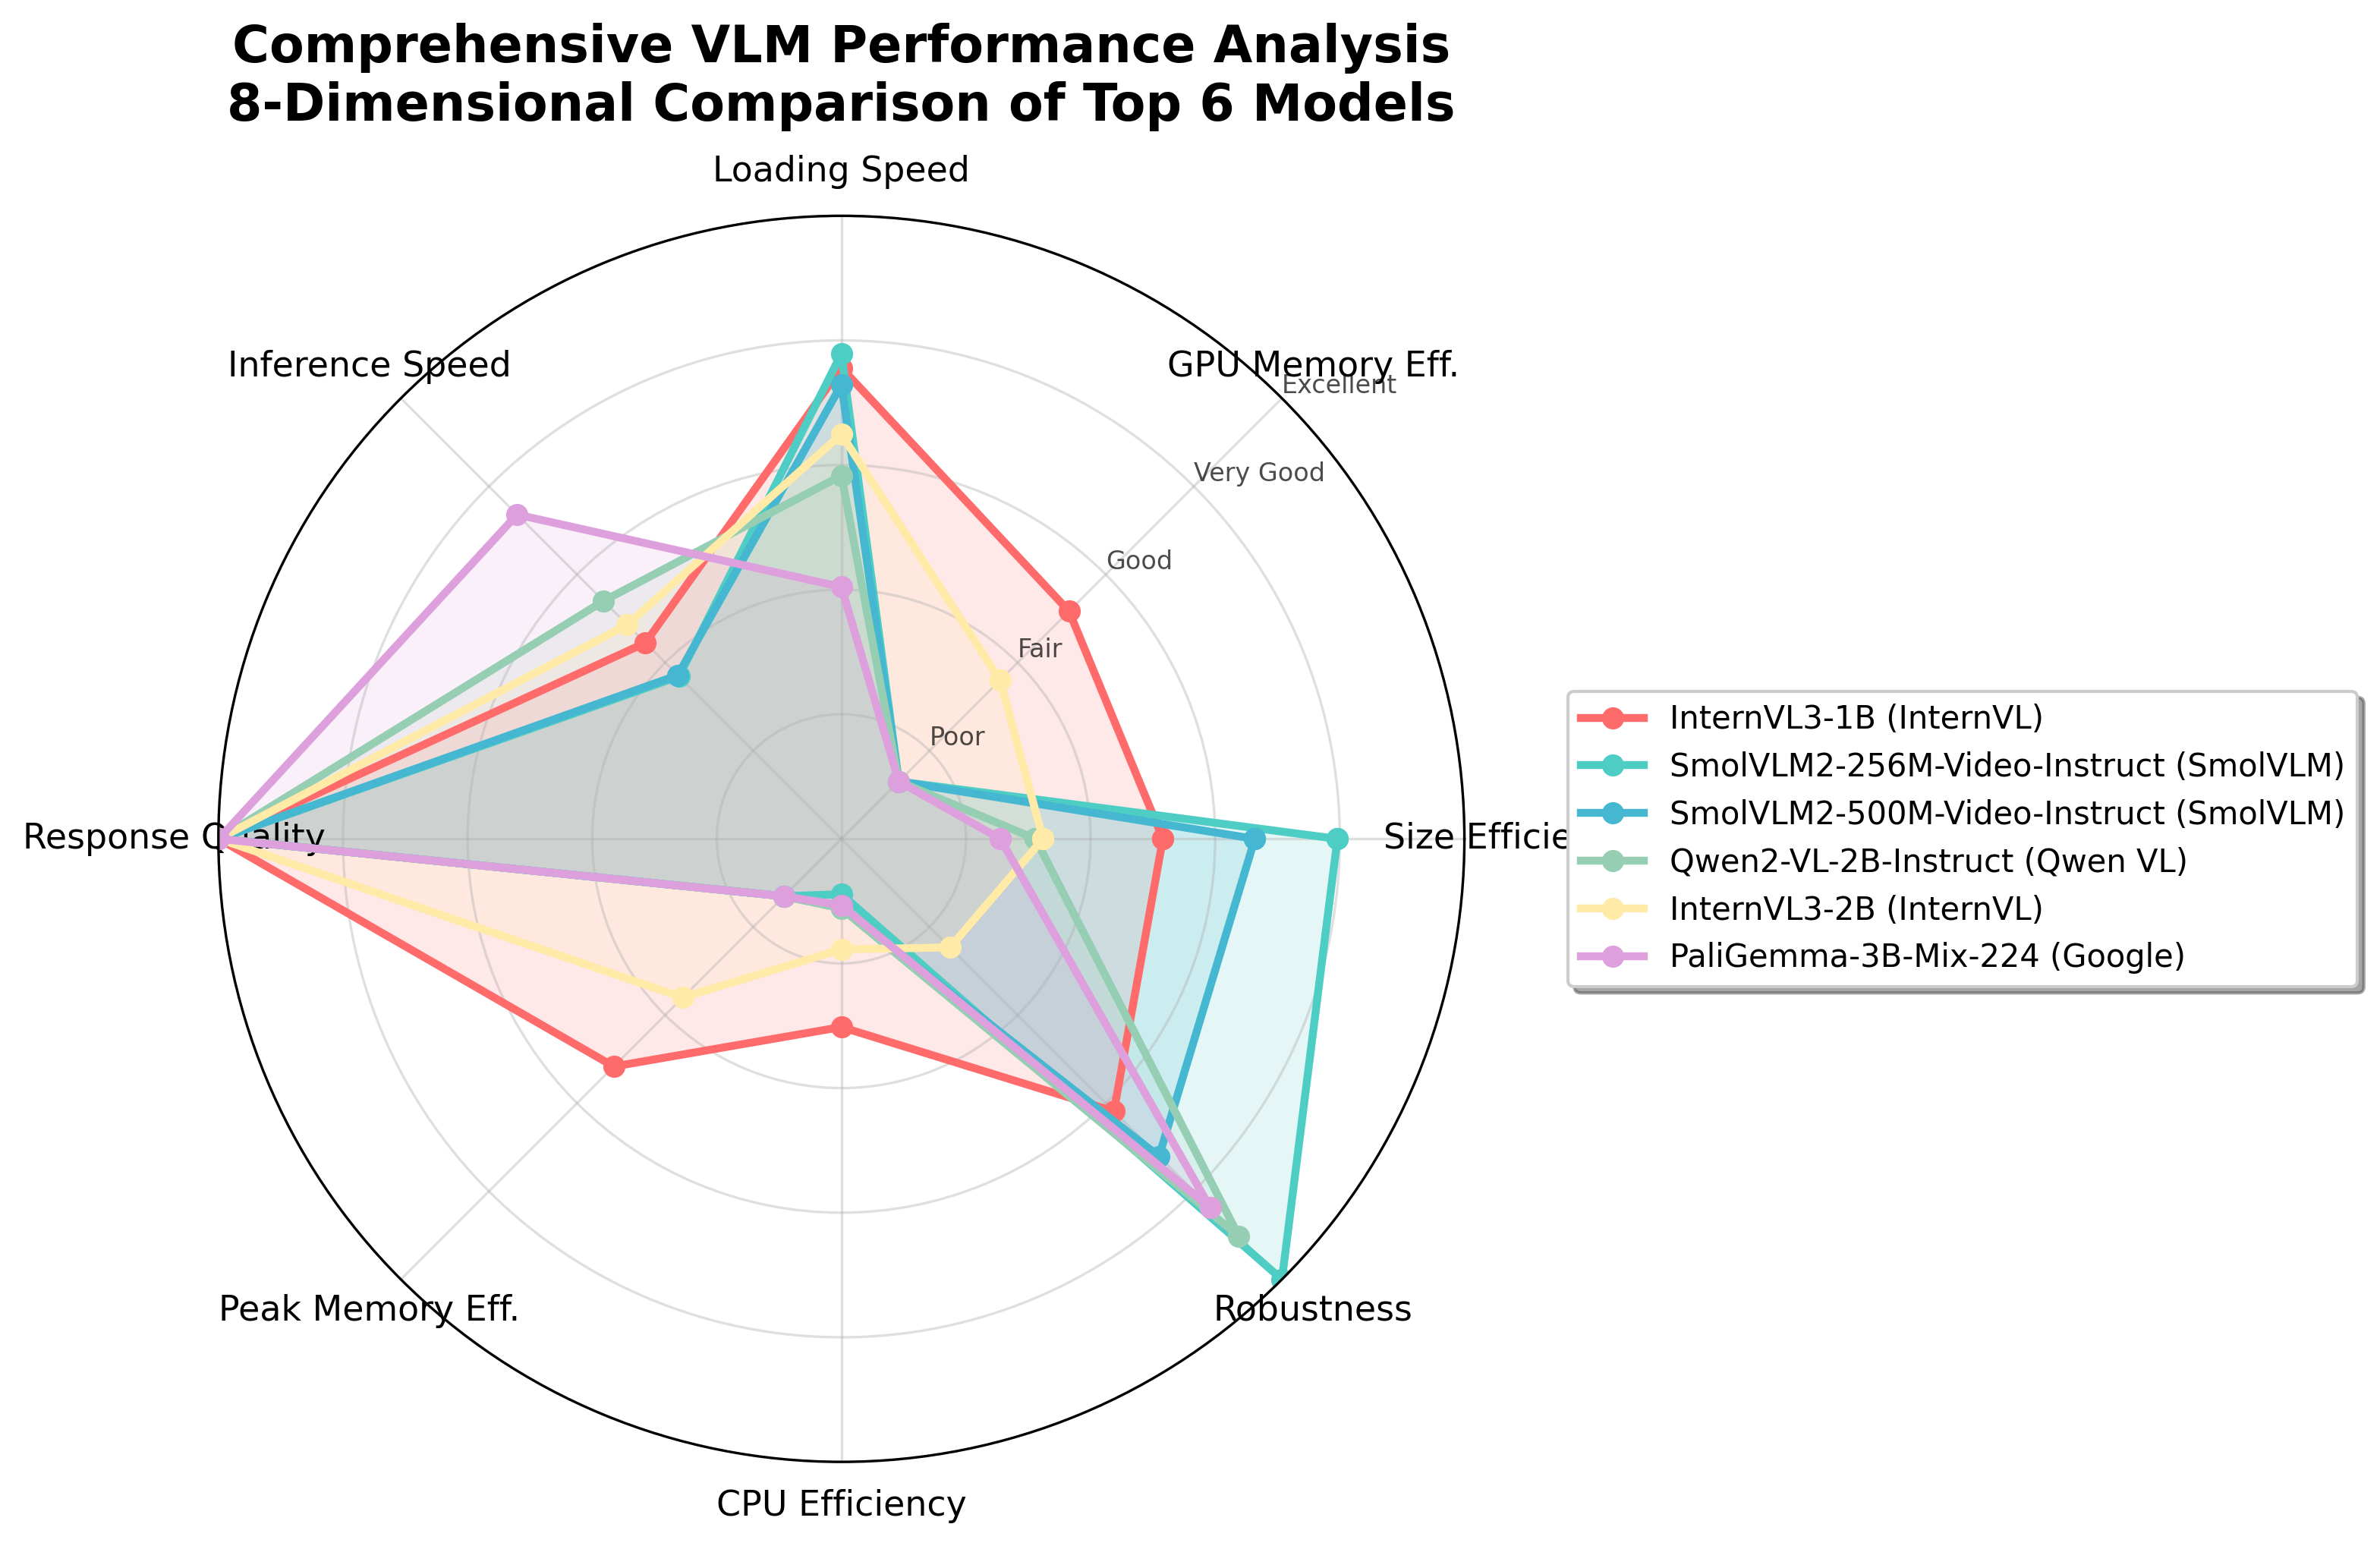
\includegraphics[width=0.9\textwidth]{figures/13_top_models_radar.png}
\caption{Comprehensive 8-dimensional performance analysis of top 6 VLMs. The radar chart compares size efficiency, memory efficiency, loading speed, inference speed, response quality, peak memory efficiency, CPU efficiency, and robustness. No single model dominates all dimensions.}
\label{fig:radar_analysis}
\end{figure*}

\subsubsection{Attack Generation Metrics}

Figure~\ref{fig:attack_metrics} analyzes the relationship between attack generation characteristics and their effectiveness.

\begin{figure*}[!t]
\centering
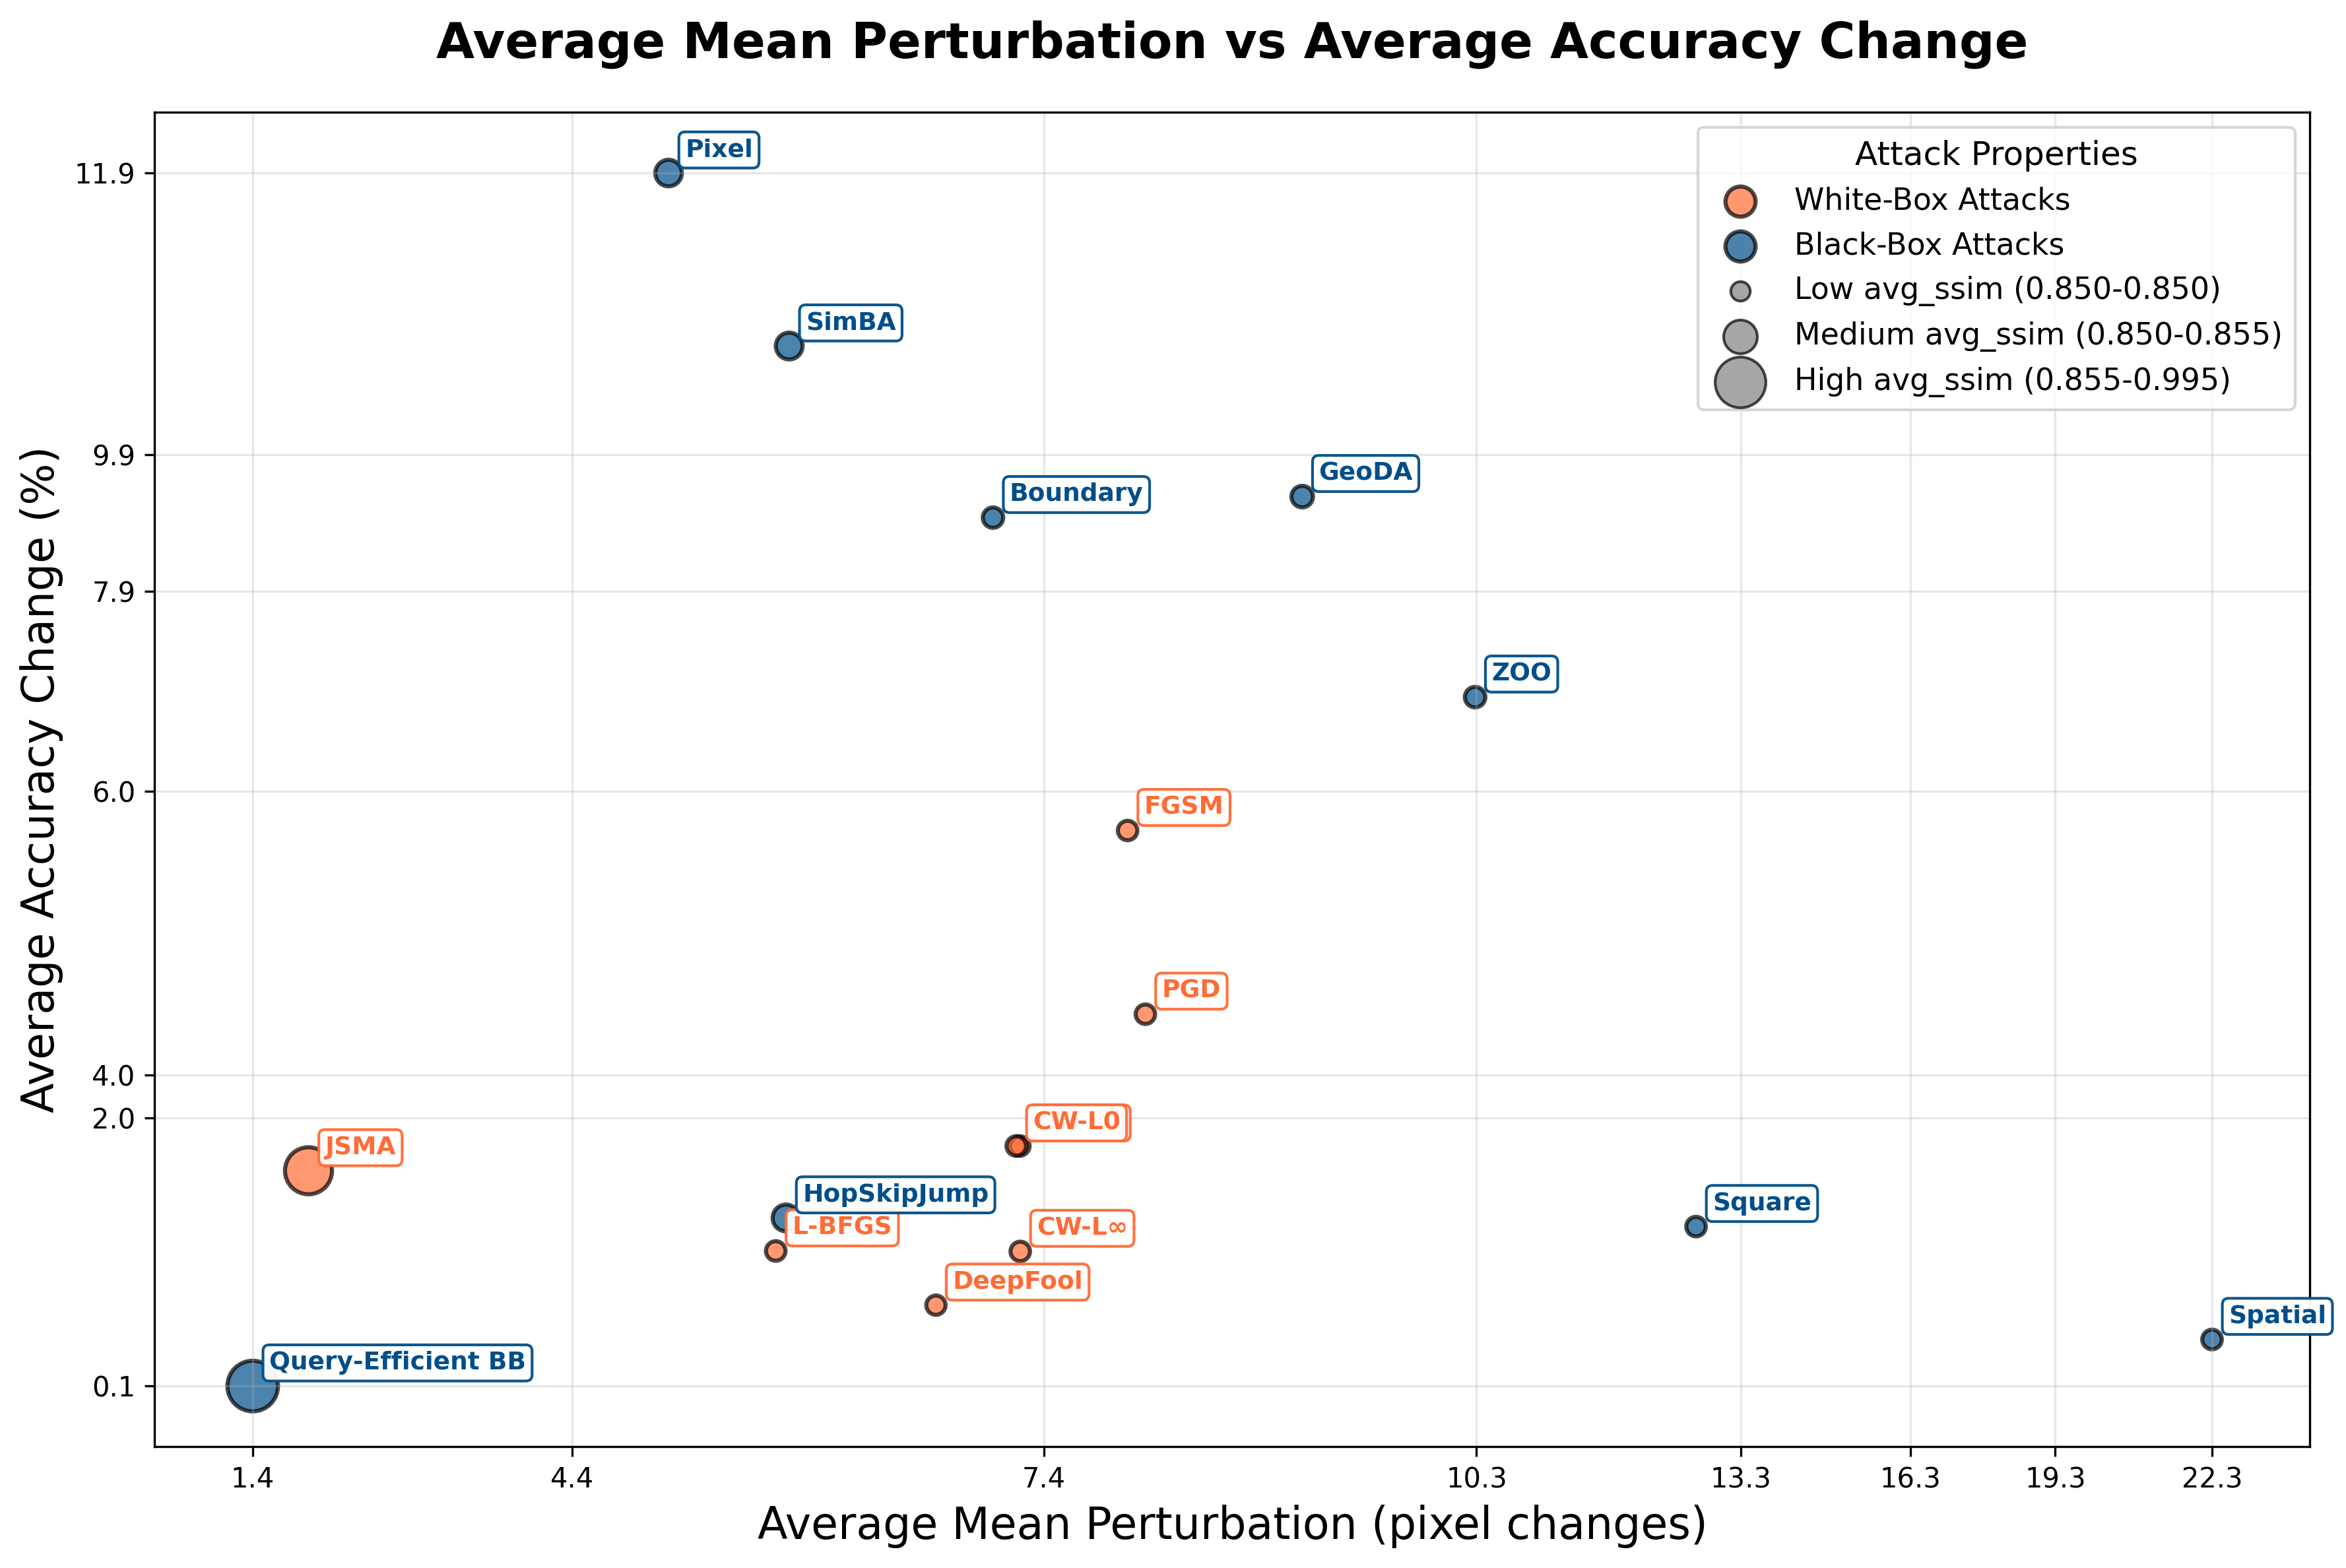
\includegraphics[width=0.9\textwidth]{figures/15_attack_raw_metrics_comparison.png}
\caption{Attack generation analysis showing the relationship between mean perturbation and accuracy change. Bubble size indicates SSIM values. The analysis reveals optimal perturbation ranges for maximum effectiveness while maintaining visual similarity.}
\label{fig:attack_metrics}
\end{figure*}

Key insights from attack generation analysis:
\begin{itemize}
    \item \textbf{Efficiency clusters}: Attacks cluster into distinct effectiveness-perturbation regions
    \item \textbf{Visual quality trade-offs}: Higher SSIM (better visual quality) correlates with lower attack effectiveness
    \item \textbf{Optimal perturbation ranges}: Most effective attacks operate within specific perturbation ranges
\end{itemize}

\subsection{Summary of Key Results}

Our comprehensive evaluation reveals several critical findings:

\begin{enumerate}
    \item \textbf{Universal vulnerability}: All 16 evaluated VLMs show significant susceptibility to adversarial attacks, with no model achieving robust performance across all scenarios.

    \item \textbf{Attack method hierarchy}: White-box attacks consistently outperform black-box methods, with PGD and AutoPGD achieving the highest success rates.

    \item \textbf{Non-linear scale effects}: Larger models do not necessarily exhibit better robustness, with optimal performance observed in the (1-2]B parameter range.

    \item \textbf{Architecture-specific patterns}: Different model families exhibit distinct vulnerability signatures, suggesting that architectural choices significantly impact robustness.

    \item \textbf{High transferability}: Adversarial attacks transfer effectively across different VLM architectures, indicating fundamental vulnerabilities in current multimodal approaches.
\end{enumerate}

These results highlight the urgent need for robust VLM architectures and defense mechanisms, particularly as these models are increasingly deployed in safety-critical applications.